\chapter{Modular approach in grasp planning}
\label{cha3}

\section{Introduction}
\label{cha3:sec1}
%%%%%%%%% TODO: extend this to unfamilar object %%%%%%%%%


Given an object and a multi-fingered robotic hand,
generating a set of contacts on the object's surface which ensure grasp stability while being feasible for the hand kinematics is a common problem in grasp synthesis. Over the last few decades, robot grasping has been a popular topic and numerous approaches for grasp planning have been proposed~\cite{sahbani2011overview}. Most of these approaches adopt iterative methods, which are usually able to find a solution within a finite number of iterations and the average computation time is usually in the range of a few to tens of seconds. However, the number of iterations required grows quadratically with the size of the problem and this creates an uncertainty of the time for the robot to plan a grasp. The upper bound of the computation time is barely analyzed in the literature.

%However, most of these approaches adopt iterative methods, which are usually computationally expensive due to the high-dimensionality of the configuration space and the non-linearity of the problem constraints. They are generally able to find a solution, sometimes within a finite number of iterations. Further, they generally try to solve the grasping problem in a static environment. Few of them consider a dynamic environment.

Moving from the traditional engineering environment into a human dominated environment necessitates a fast grasp planning strategy to respond in real time. For example, when reaching out to grasp an object, a robust grasping strategy must be able to adapt rapidly to external perturbations that can modify the initial object position and orientation relative to the robot hand. In the case of catching a flying object~\cite{kim2012}, the robot has only a few milliseconds to plan a grasp before the object touches the floor.

Another application is receiving objects handed over by humans with a robot hand~(Fig.~\ref{handover}). In many circumstances the object must be grabbed quickly: one such example is when the object is heavy or hot; other examples involve time-pressing situations, e.g. in surgery a robot assistant must react sufficiently quickly to doctors handing back implements to ensure smooth running of the surgery.

Besides human-robot interaction, real time planning for the pick-and-place task in the industrial environment may also be necessary: spare parts could be randomly placed on the conveyor belt.
The conveyor belt runs constantly at a high pace and leaves no time for the robot to stop its action and replan.
The robot must therefore respond swiftly to avoid incurring delays in production. Given the limited computational power available in computers embedded in the robot, a computationally expensive algorithm would result in a prohibitively long decision time, leading to task failure in the above scenarios.

Because of the complexity of the problem, real time grasp planning has not been extensively studied. To tackle this problem, we propose a closed-form solution which requires at most three steps to compute a new grasp, and hence guarantee a short computation time and the uncertainty is reduced to the largest extent. In this chapter, we first present a real time grasp planning strategy for familiar objects (Section~\ref{cha3:sec2},~\ref{cha3:sec3}). We then present an extension of this method to plan grasps for novel objects.


%constantly running conveyer belt to deliver to the robot, which does not stop to let the robot plan the grasps. With the limited computational power of an embedded robot computer, a computationally expensive algorithm would result in a prohibitively long decision time, leading to task failure in the above scenarios.

%In many real world scenarios, a rapid grasp planning strategy is required. For example, when reaching out to grasp an object, a robust grasping strategy should be able to adapt rapidly to external perturbations that can modify the initial object position and orientation. In catching a flying object~\cite{kim12}, the robot has to plan a grasp within a few milliseconds before the object touches the floor. Another major application is human handing over objects to robots ~(Figure~\ref{handover}). Human would normally expect their partners to grab the object quickly, especially when the object is heavy or hot. In fact, in many occasions tasks are time-pressing, e.g. in a surgery the doctors hand over tools to the robot assistant and the robot has to react sufficiently quickly to keep the surgery running smoothly. Besides human-robot interaction, real time planning for the pick-and-place task in the industrial environment is also necessary: spare parts could be randomly placed on the conveyer belt to deliver to the robot, which does not stop to let the robot plan the grasps. With limited computational power of an embedded robot computer, a computationally expensive algorithm will have a long decision time and could lead to task failure in the above scenarios.

\begin{figure}
  \centering
  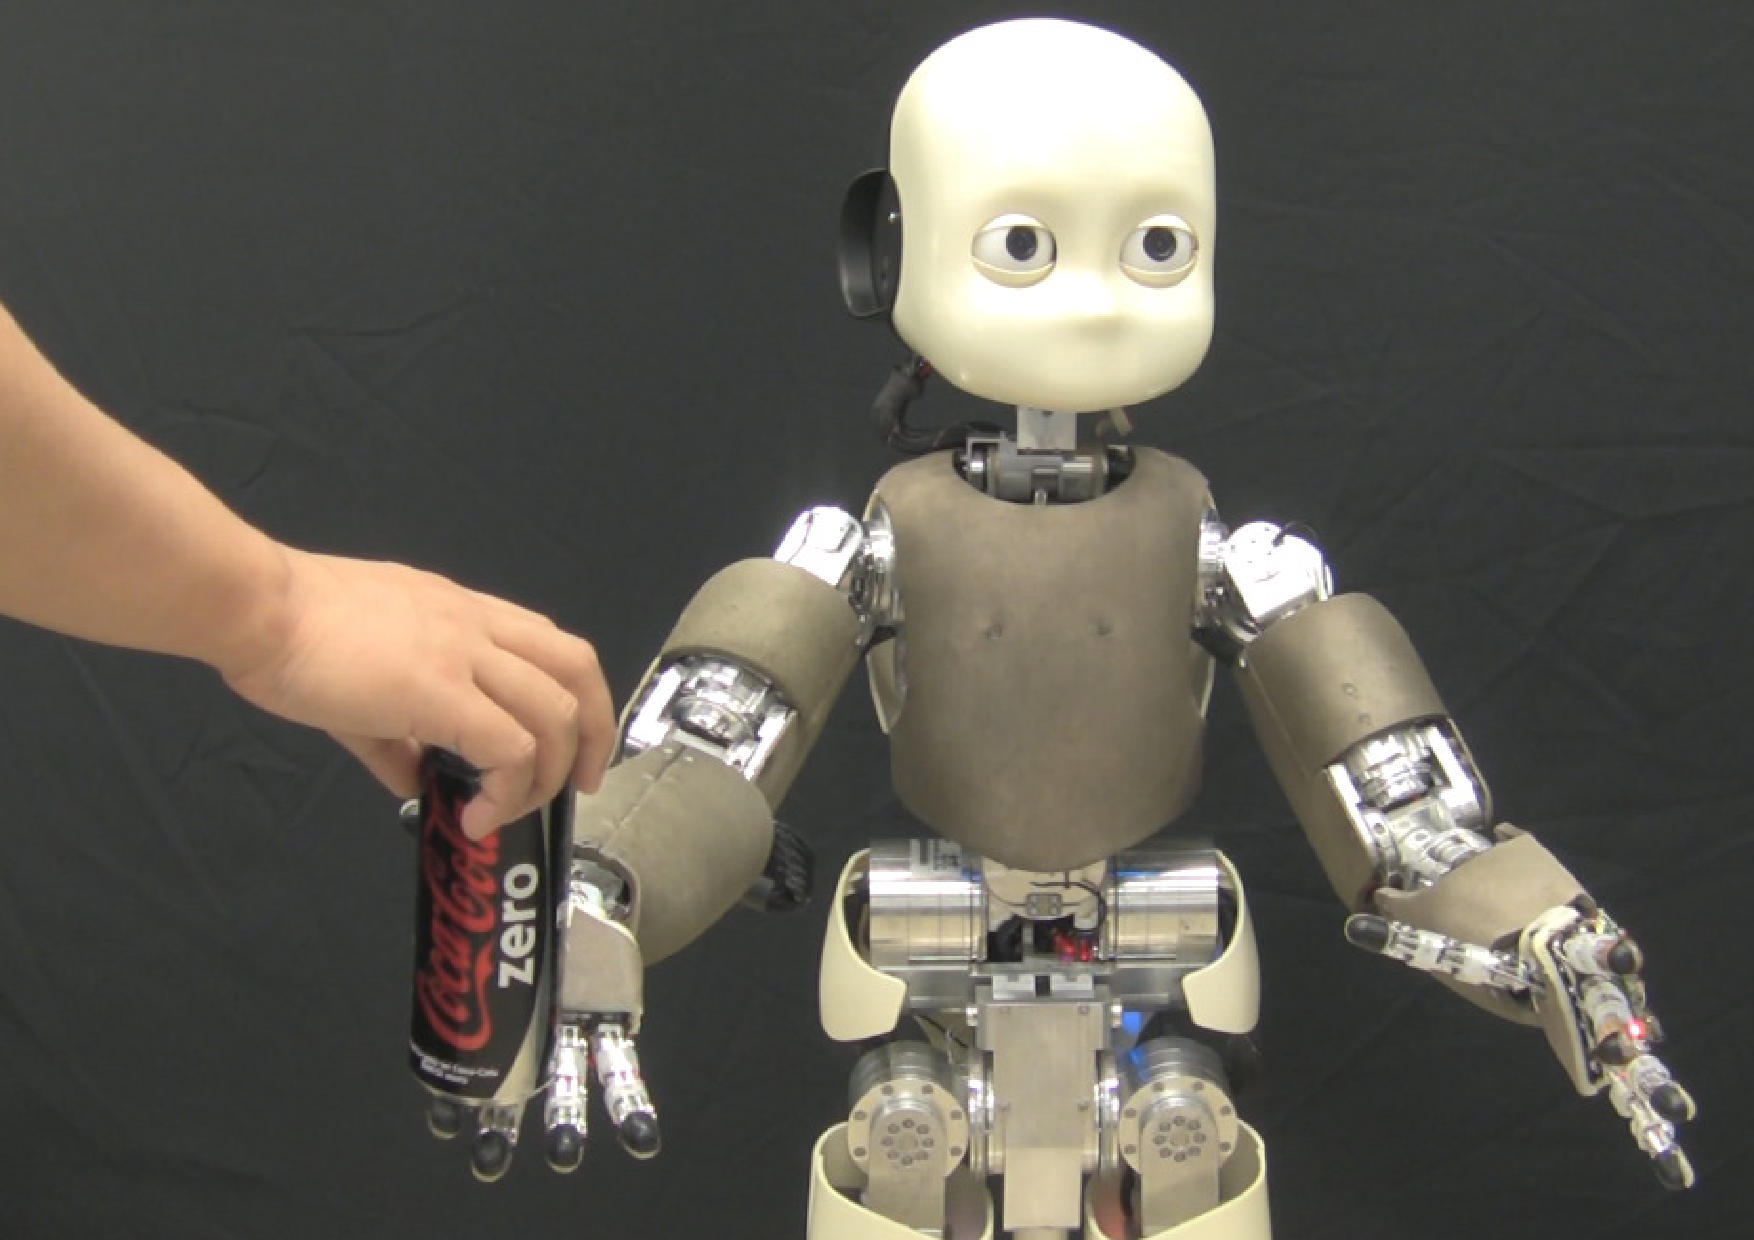
\includegraphics[width=12cm]{./fig_cha3/handover.pdf}
  \caption{A human hands a can to an iCub}
  \label{handover}
\end{figure}



\section{Fast grasp planning for familiar objects}
\label{cha3:sec2}

Traditional manipulation planning strategies usually involve inverse kinematics and optimization, which are computationally expensive. The reported computation time varies from 0.1$sec$ to a few minutes. Recently, there have been some attempts to tackle the problem with real time solutions. \citet{Richtsfeld2008} use a laser scanner to detect cylindrical shapes and plan grasps. This method is limited to cylindrical objects. Kanehiro et al.~\citep{harada2008fast} use approximation models of the friction cone and roughly estimate the force closure criterion. However, this approximation may limit their solutions. In the planning step, they use random sampling techniques to generate grasping postures and loop through the samples to find a grasp satisfying all the kinematic constraints. The reported computation time varies from 10$sec$ to 25$sec$ including path planning of the arm using a 2GHz core.
Daoud et al.~\citep{daoud2011fast} employ a genetic algorithm optimization approach to provide an initial grasp before online manipulation. This evolutionary approach relies on several iterations of optimization before reaching the solution. The reported time is 12.61$sec$ for a spherical object with a 2.2GHz core. The latter two methods, due to their iterative approaches, do not guarantee fast computation in all cases. In contrast, with our closed-form solution the computation time is bounded within a few milliseconds.

We avoid using these by adopting a learning approach.
Our method for planning grasps for familiar objects starts by generating a training dataset of stable grasps for the objects. A $Gaussian$ $Mixture$ $Model$ (GMM)~\citep{cohn1996active} is learned from the data, and the target pose is predicted via $Gaussian$ $Mixture$ $Regression$ (GMR). Hence there is no inverse kinematics computation nor iterative optimization in our method. Generally speaking, our approach is to:
\begin{enumerate}
\item Generate a set of stable grasping demonstrations for a given object and a robot hand (Section~\ref{cha3:sec2:demonstration}).
\item Build a statistical model for the training dataset offline (Section~\ref{cha3:sec2:learn}).
\item Use the model to quickly generate a new grasp, given a starting object-hand configuration (Section~\ref{cha3:sec2:plangrasp}).
\end{enumerate}

\subsection{Grasp generation given the hand kinematics}
\label{cha3:sec2:demonstration}

Two robot platforms available in our lab are chosen to perform the grasping tasks: the iCub and the Barrett hand. The iCub has an anthropomorphic hand with 9 degrees of freedom: 3 in the thumb, 2 in the index, 2 in the middle finger, 1 in the ring and little fingers and 1 for the adduction/abduction movement (Figure~\ref{fig:robothand}(a)). The Barrett hand is an industrial grasper with 3 fingers and 4 degrees of freedom: 1 for each finger and 1 for the separation between the second and the third finger (Figure.,~\ref{fig:robothand}(b)). These two platforms differ drastically in the range of motion for each finger and provide very different grasp demonstrations. They will hence grasp objects in very different ways.

\begin{figure}
  \centering
  \subfloat[\scriptsize{iCub hand}]
  {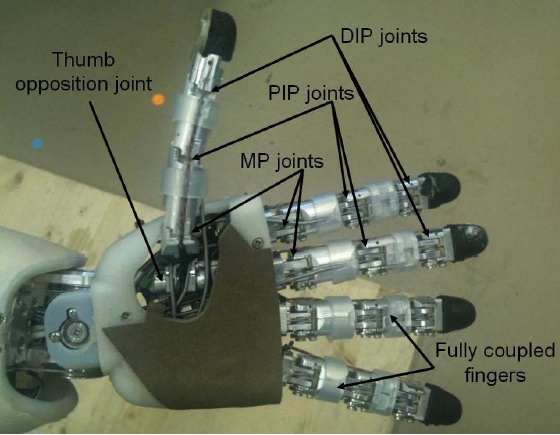
\includegraphics[height=4.5cm]{./fig_cha3/icubhand.jpg}}
  \subfloat[\scriptsize{Barrett hand}]
  {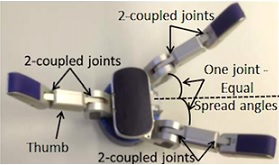
\includegraphics[height=4.5cm]{./fig_cha3/barretthand.jpg}}
  \caption{Two robot platforms used in this work. This method is not bounded to these two robots. It can be applied to any other robot hands given their kinematics.}
  \label{fig:robothand}
\end{figure}

Starting from the geometry of an object and the kinematic property of a robot hand to compute a feasible grasp is time consuming. To achieve fast planning, we do this computation offline. There are numerous possible ways to grasp one object depending on the task's needs~\citep{sahar2012,el2013generation}. To encapsulate all the possible ways, a large amount of training data is needed. Collecting this amount of data on a real robot is time consuming. Therefore, instead of using a real robot, we generate training data by synthesis.

Two different approaches are used here: optimization and simulation. We use a simulation method for the Barrett hand and an optimization method for the iCub hand. In simulation, we use a trial-and-error approach: in the state space we try to generate as many grasps as possible and select those feasible ones. In principle we can generate more variety of grasps by this method, as some of them might be hard to reach by optimization. The 4 d.o.f Barrett hand is particularly suitable for this approach. For the 14 d.o.f iCub hand, however, the state space is much larger and hence the trial-and-error approach is expensive. Instead, for the iCub hand we use an optimization method.


%\subsubsection{Optimization}
\paragraph{Optimization}
~\\
We use the optimization algorithm proposed in the work of El-Khoury and etc.~\citep{el2013generation} to generate grasps for the iCub.
The iCub hand is modelled in 8 dimensions in this algorithm and the thumb, index and middle finger are taken into account.

This optimization algorithm formulates the problem as a constraint-based minimization for a set of hand configuration parameters (hand position \textbf{\emph{h}}, hand orientation {\textbf{\emph{o}}} and finger joints {\boldsymbol{$\theta$}}). These parameters are subjected to a number of constraints to satisfy the following criteria:

\begin{enumerate}
\item The grasp is kinematically feasible for the robot hand;
\item The grasp is a force-closure grasp;
\item The robot hand is not penetrating the object;
\item The robot fingertips contact the object surface;
\item The force provided by the robot hand is able to raise the object.
\end{enumerate}


The iCub's finger joints can only apply a limited amount of torque.
The less joint torque required, the easier it is for the iCub to lift the object. For this reason, we choose the objective function to be the minimum joint torque required to balance the gravity wrench, formulated as:
\begin{equation}
J(\boldsymbol{h},\boldsymbol{o},\boldsymbol{\theta})=\Arrowvert \sum_{i,j} {{\tau}^j_i}\Arrowvert
 \label{quality}
 \end{equation}
where {$\tau$}$^j_i$ is the $i$th joint torque of the $j$th fingers under the force feasibility constraints:

\begin{equation}
 {\tau}^j_i \in [\bar{\tau}^j_i, \hat{\tau}^j_i]
 \label{quality}
\end{equation}
where $\bar{\tau}^j_i$ and $\hat{\tau}^j_i$ are the lower and upper boundaries of $\tau^j_i$.
Minimizing this cost function is equivalent to minimizing the energy required in the joint space in order to accomplish the grasping task.
%As different grasps can cost similar amounts of energy, this objective function has many local optima and hence can provide a large set of different grasps.

The optimization is solved by the Interior Point OPTimizer (IPOPT) method proposed by W\"{a}chter and Biegler~\citep{wachter2006implementation}, written in the AMPL Model Language for Mathematical Programming. To generate a variety of grasps, we exploit the fact that the IPOPT solver converges to local solutions. We provide the solver with a large number of initial conditions, varying from 1000 to 2000. From these initial conditions, which are located in different areas of the space, the IPOPT converges to their corresponding local optima. By this means 500 to 1000 optimized grasps for an object can be obtained. They will be used as the training data in the next phase. The average computation time for the IPOPT to converge to one solution is 2.65$sec$, with a standard deviation of 1.82$sec$. As additional information, the quality $Q$ of each optimized grasp is calculated in the form described in~\citep{ponce1997computing}:

\begin{equation}
Q =\Arrowvert \frac{1}{3}\sum_{j} {\boldsymbol{c}^j}\Arrowvert
\vspace{-0.1in}
\end{equation}
where \textbf{\emph{c}}$^j$ is the contact point (i.e. fingertip) position of the $j$th finger. Though it is not included in the optimization, the quality is used in the comparison between the training set and the result set shown in Section~\ref{cha3:sec3}.
%\textcolor{red}{I don't understand how you can sum the contact points (positions as vectors?), to achieve a quality metric. Maybe the commented out text below provides the explanation required here?}
%, by the distance from the grasp polyhedron to the center of mass of the object:

%To measure the quality of the optimized grasps, the quality $Q$ is calculated as described in~\citep{ponce1997computing}, by the distance from the grasp polyhedron to the center of mass of the object:

To ensure the robot fingertips contact the object surface, the object has to be expressed by an implicit equation. For example, a cylinder can be expressed as:

\begin{equation}
{\left(x^2+y^2\right)}^{10}+z^{20} = 1
 \label{equ:cylinder}
\end{equation}

This expression is in the form of superquadrics, which will be explained in detail in the Section~\ref{cha3:sec4:pgdistribution}.

During optimization, this will be used as a hard constraint for the all the fingertip positions.
For more complex shapes, the implicit equation can be learned by a Gaussian process~\citep{el2013generation}.

The algorithm above can generate a variety of high quality force-closure grasps for a given robot hand kinematic structure and an object model. Since IPOPT is a continuous optimization solver, generating grasps on complex objects requires a continuous implicit representation of the whole object surface model.

%Representing complex objects as an assembly of superquadrics induces a discontinuity in this model preventing IPOPT from converging to a feasible solution.
%An implicit object representation for grasp generation using optimization will be addressed in our future work. This paper will only focus on grasps generated, for the iCub hand, on simple shaped objects such as a cylinder and cuboid.



%\subsubsection{Simulation}
\paragraph{Simulation}
~\\
%TODO: quality criterion: Ferrari and Canny
As the Barrett hand is modelled in the widely used simulator GraspIt!~\citep{miller2004graspit}, we use simulation to generate its data. GraspIt! is designed for grasp analysis and it provides a library of robots and object models. Its quality measurement module computes the grasp quality according to all the contacts between the hand and the object, in the form described by Ferrari and Canny~\citep{ferrari1992planning}. A grasp planning module for primitive shapes, i.e cylinder, sphere, cuboid and cone, is available, allowing users to easily generate grasps~\citep{miller2003automatic}.
To sample grasps for objects with complex shapes, we alter the module and generate grasps as follows.

\begin{figure}
  \centering
  \subfloat[\scriptsize{Initial distribution}]  {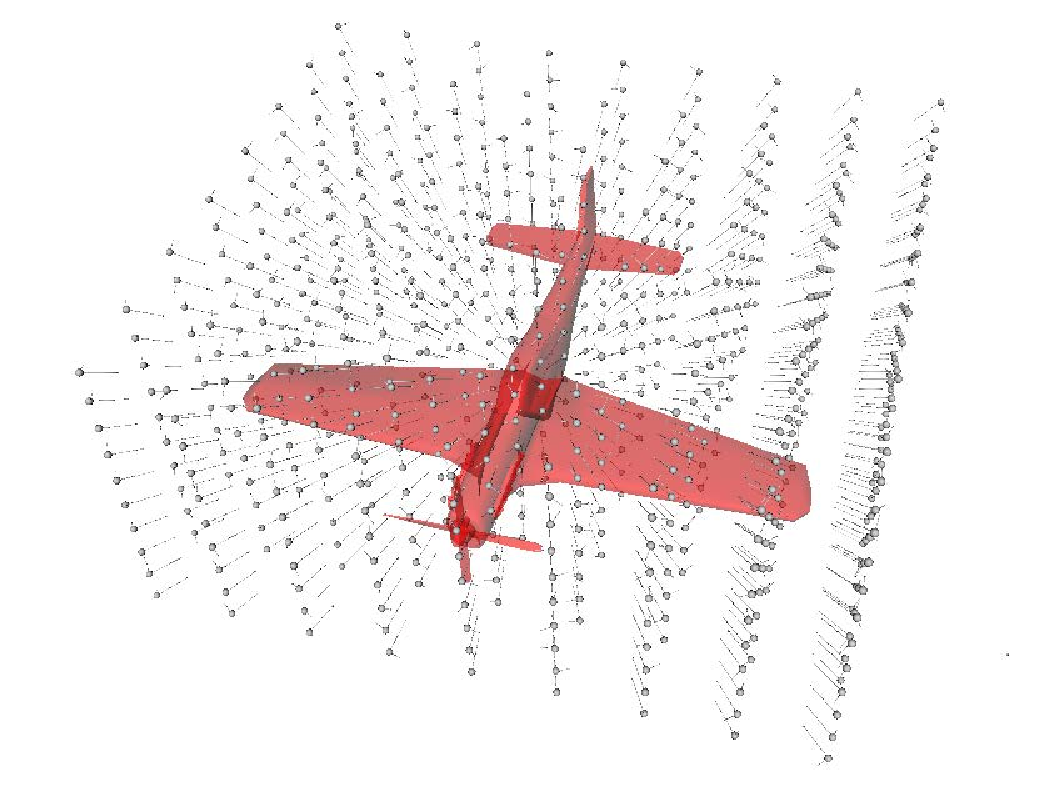
\includegraphics[width=7cm]{./fig_cha3/plane_x2_lattice1.pdf}}
  \subfloat[\scriptsize{Final distribution}]  {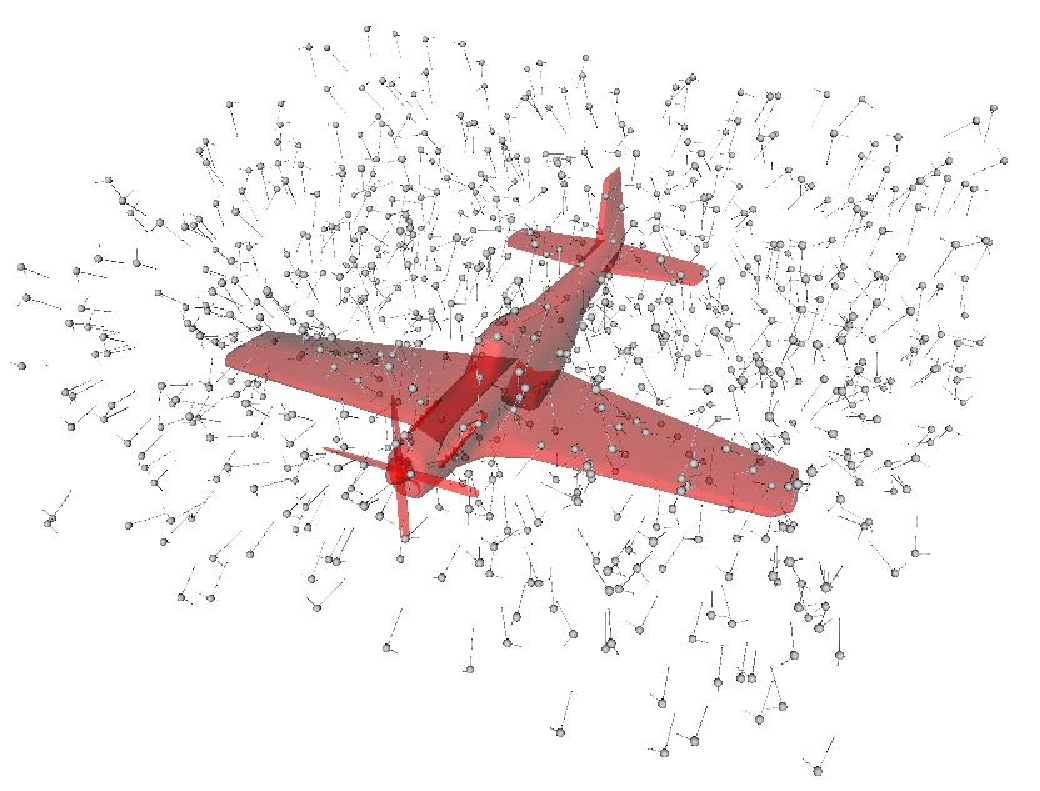
\includegraphics[width=7cm]{./fig_cha3/plane_x2_lattice2.pdf}}
  \caption{\scriptsize{An illustration of part of the grasp position lattice of an aeroplane model. Each grey dot in the lattice represents one robot hand position. The long arrows at each dot represent the hand normal directions and the short arrows represent the fix finger directions. The hand normals are initialized by pointing toward the center of the object, as shown in (a). A small random variance is then added to each grasp later to even the distribution and the final distribution is shown in (b).}
}
    \label{lattice}
\end{figure}

Firstly a robot hand position ``lattice" is generated. Each vertex in the lattice represents one robot hand position, where the hand will be placed to grasp the object (Figure~\ref{lattice}). The object is located in the center of the lattice surrounded by the grasping positions. All palm normals are initially pointing to the center of the object. Random finger separation angles are assigned to each point to form a list of grasp configurations for testing. According to the object size, 1000 to 20000\footnote{More complex and bigger shapes need more testing points.} testing grasps can be generated to ensure that the entire object is surrounded by the lattice and the farthest point to grasp the object is included. The density of the hand position lattice depends on the object shape. Objects with sharp edges, where the normals on the surface change sharply, should have a higher lattice density compared to those with smooth surfaces.

In the final step before testing, small random perturbations are added to each grasp so that the testing points are evenly and continuously distributed in all dimensions.
To test these grasps, the hand is first placed at each position on the test list with the desired posture (hand orientations and finger joints). Next, the fingers clutch around the object until contacts or joint limits prevent further motion. We then use the quality measurement module to compute the quality of each grasp. The non-zero quality grasps, i.e. force-closure grasps, are recorded and used as training data. Note that not all the testing grasps result in feasible grasps. Points causing collisions are removed from the list and only the force-closure grasps are kept as the training data. The average generating rate for the feasible grasps is roughly one per five seconds.

The Barrett hand has one joint in each finger. These three joints can only rotate in one direction and how much they rotate is determined by the object surface, given the hand position, orientation and the separation angle.
Therefore we drop this redundant information and model a Barrett hand grasp only with the hand position, hand orientation and the finger separation angle. The robot kinematics is programmed into the simulator and all simulated robot movement is feasible.

The above two methods can be used to generate both simple shapes and complex shapes. The size of the generated training data varies from 500 to 1600 (Table~\ref{result}). Each training dataset is split into 5 groups for the 5-fold cross validation in the later step.


\subsection{Model learning}
\label{cha3:sec2:learn}

The second phase of the approach is to build a model $\varOmega$ for the grasp demonstrations.
A $Gaussian$ $Mixture$ $Model$ (GMM) is used here to get a probabilistic encoding of the joint distribution $p$(\textbf{\emph{h}},\textbf{\emph{o}},\textbf{\emph{$\theta$}} \text{\textbar} $\varOmega$).
We choose to use GMM because of its ability to effectively extrapolate the missing data, as has been exploited in many applications~\citep{calinon2007learning,sauser2011iterative}. It also has the advantage of capturing the non-linearity of the space, as well as determining how likely a point in the input space is under the model.
The ability to estimate the likelihood of an input query point is crucial: an inference far away from the region covered by the training data can be unreliable, resulting potentially in an infeasible grasp. With GMM we are able to make sure that each input query point is located in or projected to a reliable region (this is explained in the next phase).

Therefore, in the grasp planning phase, we first make sure that a new query point locates in a reliable region by checking its likelihood.
Given a set of sample grasps represented by the hand position \textbf{\emph{h}},  orientation \textbf{\emph{o}} and the finger configuration \boldsymbol{$\theta$}, we model the distribution with a GMM as a sum of $K$ Gaussian components:

%$\xi$\{{\bf {\em h}},{\bf {\em o}},{\boldmath$\theta$}\}, we build our statistical model as a GMM:

\begin{equation}
{
P (\boldsymbol{h},\boldsymbol{o},\boldsymbol\theta \text{\textbar} \varOmega)
= \sum_{k=1}^K {p_{k}p(\boldsymbol{h},\boldsymbol{o},\boldsymbol{\theta} \text{\textbar} {\boldsymbol{\mu}_k}, {\boldsymbol{\Sigma}_k})}
}
\end{equation}
where $k$ is the number of Gaussian components, $p_k$ the prior of the Gaussian component and the $\boldsymbol{\mu}_k$, $\boldsymbol{\Sigma}_k$ the corresponding mean and covariance as:

\begin{equation}
{
\boldsymbol{\mu}_k = \begin{pmatrix}    \boldsymbol{\mu}_{h,k}     \\
                                        \boldsymbol{\mu}_{o,k}          \\
                                        \boldsymbol{\mu}_{\theta,k}
                    \end{pmatrix}
\hspace{0.2in}
\boldsymbol{\Sigma}_k = \begin{pmatrix}     \boldsymbol{\Sigma}_{hh,k}  & \boldsymbol{\Sigma}_{ho,k} & \boldsymbol{\Sigma}_{h\theta,k}  \\
                                            \boldsymbol{\Sigma}_{oh,k}  & \boldsymbol{\Sigma}_{oo,k}  & \boldsymbol{\Sigma}_{o\theta,k} \\
                                            \boldsymbol{\Sigma}_{\theta{h},k}   & \boldsymbol{\Sigma}_{\theta{o},k}   & \boldsymbol{\Sigma}_{\theta{\theta},k}
                        \end{pmatrix}
}
\end{equation}

A GMM approach requires that the data space is locally convex. For a complex object shape, however, the grasp space of hand configuration --- coupled with the finger joint space and constrained by the geometry of the object surface --- may be a non-smooth manifold. In both of the data generation methods described above, we evenly distribute the testing points so as to reduce the possibility of missing small good grasp regions. By these means we obtain most of the possible grasps for the object and approximate a locally convex data distribution, which is suitable for a GMM.

Before training we 1) convert all data into the object reference frame and 2) normalize the data so that all dimensions have a zero mean and a unit variance. Initialized by the K-means, the $Expectation$-$Maximization$ $algorithm$ (EM)~\citep{dempster1977maximum} is used to find the value of $\boldsymbol\mu$ and $\boldsymbol\Sigma$ that maximizes the probability of the training data under the GMM. The number of Gaussian $K$ is selected by the $Bayesian$ $Information$ $Criterion$ (BIC) and verified by 5-fold cross validation to make sure the model is not overfitting (Figure~\ref{bicxv}).

\begin{figure}
  \centering
    \subfloat[\scriptsize{BIC}]  {\label{fig:reachableSamplesPos}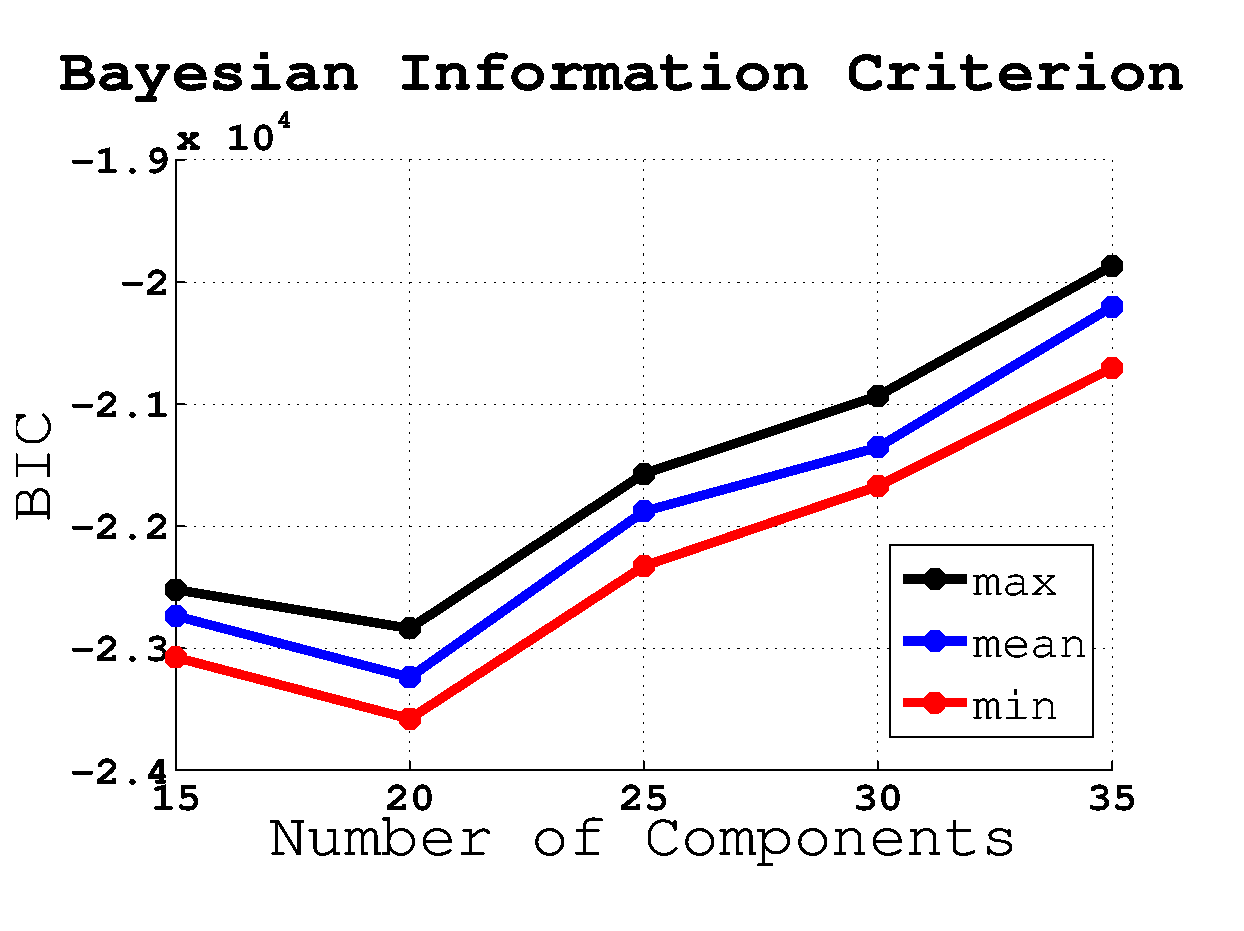
\includegraphics[width=7cm]{./fig_cha3/BIC.eps}}
    \subfloat[\scriptsize{5-fold cross validation}] {\label{fig:reachableModelPos}  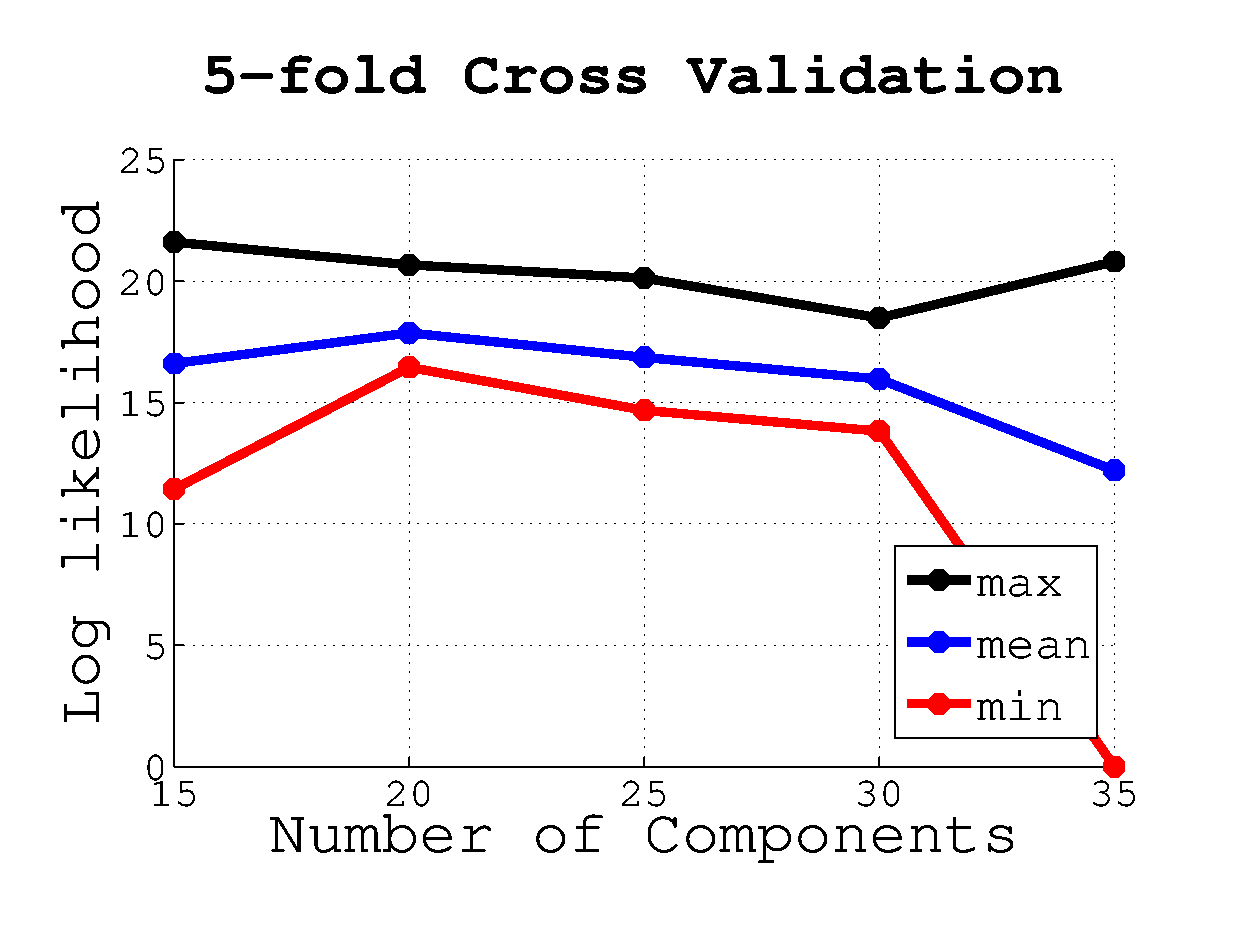
\includegraphics[width=7cm]{./fig_cha3/xValidation.eps}}

  \caption{\scriptsize{The $Bayesian$ $Information$ $Criterion$ and 5-fold cross validation test results of the training dataset of the Barrett hand and a joystick shaped object. For each number of Gaussians, the test is run 5 times. After empirical testing, the number of Gaussians is chosen to be 20. The corresponding experiment are shown in Section~\ref{cha3:sec3}.}
}
    \label{bicxv}
\end{figure}

\subsection{Grasp Planning}
\label{cha3:sec2:plangrasp}

With the learned GMM model of the grasping demonstrations, we plan a feasible grasp given a current hand configuration \textbf{\emph{q}}=\{\textbf{\emph{h}},\textbf{\emph{o}}\}. As discussed above, we first need to determine whether the \textbf{\emph{q}} is a valid query point. To do this we define a membership function $f$(\textbf{\emph{q}}) as:

\begin{equation}
f(\boldsymbol{q}) = \sum_{k=1}^{K}\bar{\boldsymbol{N}}(\boldsymbol{q};\boldsymbol{\mu}_k,\boldsymbol{\Sigma}_k)
\end{equation}
where $\bar{\boldsymbol{N}}$ is the normal distribution with the output being normalized between 0 and 1:

\begin{equation}
\bar{\boldsymbol{N}}(\boldsymbol{q};\boldsymbol{\mu}_k,\boldsymbol{\Sigma}_k) = exp\left(-\frac{1}{2}(\boldsymbol{q}-\boldsymbol{\mu}_k)^{T}\boldsymbol{\Sigma}_k^{-1}(\boldsymbol{q}-\boldsymbol{\mu}_k)\right)
\end{equation}

We consider a point to belong to the model if its Mahalanobis distance to any Gaussian component is less than a given threshold $\sigma$. In our experiments, we find that within 1~standard deviation the success rate of finding a feasible grasp is constantly high. For example in the Barrett hand and the model plane grasping task, the rate of producing a feasible and stable grasp within 1 standard deviation is 85\% (Table~\ref{result}) while it is 64\% within 3 standard deviations. On the other hand, it is possible that GMM encapsulates two different clusters of data within a single Gaussian, leaving the mean of the Gaussian at an infeasible point. This means getting closer to the means does not ensure a higher success rate. Taking this trade-off into account, we choose 1 standard deviation as our threshold, which gives us a cutoff criterion $\eta$ = $exp(-\frac{1}{2}\sigma^2)$. If the membership function of a point has a higher value than $\eta$, we consider this point as a valid query point. Note that the finger configuration $\boldsymbol\theta$ is not part of this input query point as $\boldsymbol\theta$ will be inferred by GMR later.

This membership function differs from the marginal likelihood $p$(\textbf{\emph{h}},\textbf{\emph{o}}) in two aspects. Firstly, it gives each Gaussian component the same weight, regardless of their priors $p_k$. As the prior of each Gaussian is proportional to the number of data points that are explained by this Gaussian, using this information in our selection may bias our choice toward the ``most popular" grasps, yielding less variety in the results.
Secondly, $\bar{\boldsymbol{N}}$ is a normalized function bounded between 0 and 1. This ensures the points with the same Mahalanobis distance from a Gaussian will have the same membership value, regardless of the size of the covariance~\citep{sauser2011iterative}.


In the case that \textbf{\emph{q}} is not a valid query point, we need to project it to a new point $\boldsymbol{q}^*$ that has a membership function value higher than $\eta$. Here we use a closed-form solution by considering each individual Gaussian component. We first compare the Mahalanobis distances between the query point \textbf{\emph{q}} and each Gaussian to find the nearest Gaussian component. The projection point $\boldsymbol{q}^*$ is found by projecting $\boldsymbol{q}$ to this nearest component (Figure~\ref{contour}).
%Point \textbf{\emph{q}} is then projected to this component to find the nearest point $\boldsymbol{q}^*$, which is less than one standard deviation away from the center of the Gaussian (Figure~\ref{contour}).
In the Mahalanobis space the Gaussian is in a uniform shape. As a result, the projection point $\boldsymbol{q}^*$  lays on the direction from the \textbf{\emph{q}} to the center of the Gaussian. Therefore the projection point $\boldsymbol{q}^*_k$ of the $k^{th}$ Gaussian can be written as:


\begin{equation}
\boldsymbol{q}^*_k = \boldsymbol{q} + \alpha_k(\boldsymbol{q}-\boldsymbol{\mu}_k)
\end{equation}
where $\alpha_k$ is a scalar. With $\sigma = 1$ and the equation

\begin{equation}
\bar{\boldsymbol{N}}_k(\boldsymbol{q};\boldsymbol{\mu}_k,\boldsymbol{\Sigma}_k) = exp(-\frac{1}{2}\sigma^2)
\end{equation}
we have the equation to easily compute $\boldsymbol{q}^*_k$:

\begin{equation}
-\frac{1}{2}(\boldsymbol{q}^*_k-\boldsymbol{\mu}_k)^{T}\boldsymbol{\Sigma}^{-1}_{k}(\boldsymbol{q}^*_k-\boldsymbol{\mu}_k) = -\frac{1}{2}\cdot{1}^{2}
\end{equation}

Once the projection point $\boldsymbol{q}^*$ is found, the $Gaussian$ $Mixture$ $Regression$ (GMR) is used to predict a feasible finger configuration $\boldsymbol\theta^*$ for it. First we define:

\begin{equation}
{
\boldsymbol{\mu}_{q,k} = \begin{pmatrix} \boldsymbol{\mu}_{h,k}    \\
                                        \boldsymbol{\mu}_{o,k}
                        \end{pmatrix}
\hspace{0.3in}
\boldsymbol{\Sigma}_{qq,k} =  \begin{pmatrix}  \boldsymbol{\Sigma}_{hh,k}  & \boldsymbol{\Sigma}_{ho,k}  \\
                                            \boldsymbol{\Sigma}_{oh,k}  & \boldsymbol{\Sigma}_{oo,k}
                            \end{pmatrix}
}
\end{equation}
and GMR then uses:

\begin{equation}
{
\hat{\boldsymbol{\mu}}_{\theta,k} = \boldsymbol{\mu}_{\theta,k} + \boldsymbol{\Sigma}_{\theta{q},k}(\boldsymbol{\Sigma}_{qq,k})^{-1}(\boldsymbol{q}-\boldsymbol{\mu}_{q,k})
}
\end{equation}

\begin{equation}
{
\hat{\boldsymbol{\Sigma}}_{\theta\theta,k} = \boldsymbol{\Sigma}_{\theta\theta,k} - \boldsymbol{\Sigma}_{\theta{q},k}(\boldsymbol{\Sigma}_{qq,k})^{-1}\boldsymbol{\Sigma}_{{q}\theta,k}
}
\end{equation}


Finally, all the $K$ components are taken into account and the target finger configuration $\boldsymbol{\theta}^*$ is predicted as the mean $\hat{\boldsymbol{\mu}}_\theta$ with the covariance $\hat{\boldsymbol{\Sigma}}_{\theta\theta}$ according to:

\begin{equation}
{
\hat{\boldsymbol{\mu}}_{\theta} = \sum_{k=1}^K{\beta_k(\boldsymbol{q}^*)}\hat{\boldsymbol{\mu}}_{\theta,k}
}
\end{equation}
\begin{equation}
{
\hat{\boldsymbol{\Sigma}}_{\theta\theta} = \sum_{k=1}^K{\beta_k(\boldsymbol{q}^*)}^2\hat{\boldsymbol{\Sigma}}_{\theta\theta,k}
}
\end{equation}
where
\begin{equation}
{
\beta_k(\boldsymbol{q}^*) = \frac{p_{k}p(\boldsymbol{q}^*|\boldsymbol{\mu}_{q,k},\boldsymbol{\Sigma}_{qq,k})}{\sum_{k=1}^K{p_k}p(\boldsymbol{q}^*|\boldsymbol{\mu}_{q,k},\boldsymbol{\Sigma}_{qq,k})}
}
\end{equation}

Due to the probabilistic nature of the GMR, the inferred result $\boldsymbol{\theta}^*$ is not a unique value but a mean value with variance. Though this mean does not guarantee a feasible solution, it provides a good estimation of a feasible one.

To find the closest Gaussian component we used the Mahalanobis distance rather than the Euclidean distance. The advantage of this is that it takes into account the correlations among each dimension of the hand configuration. In a space of different types of measurements, i.e. length and angle, Mahalanobis space is a better representation than the Euclidean space. Indeed, humans do not always use the Euclidean distance to select their grasps. We may move our hand further than needed to grasp an object, in order to avoid flipping our hand to another orientation. The performance of this method is discussed in the next section.


\section{Experiments of planning grasps for familiar objects}
\label{cha3:sec3}

This section presents a few results of our method (Figure~\ref{contour},~\ref{icub_cuboid}\footnote{The small penetrations and gaps between the fingers and the object are caused by two factors, (1) that the width of the fingers are not taken into account in the optimization and (2) the variance of the results. A supplemental implementation will be applied on the real scenario to handle the variances.},~\ref{barrett}). As mentioned above, grasps of the iCub hand are described in 14 dimensions: hand position (3D), hand orientation (3D in Euler angles) and finger joint angles (8D). Grasps of the Barrett hand are described in 8 dimensions: hand position (3D), hand orientation (4D in axis-angle representations) and finger separation angle (1D). Six different objects are presented here: cylinder, cuboid, ashtray, shoe, joystick and aeroplane model. For each object, three different initial postures and their final grasps are shown. Figure~\ref{contour} shows the results of the iCub grasping a cylinder, and the corresponding projections from the initial query points to the model. The results of the cylinder and cuboid show that a variety of grasps can be obtained for simple shapes to satisfy different task requirements. The ashtray, aeroplane model and joystick shapes are chosen from the GraspIt! object library, showing the method indeed works with complex shapes. In some figures the wrist may seem to rotate over 360 degrees to reach the final grasps from the initial pose. This is because the path planning of the arm is not taken into account in our approach. In terms of the hand orientation solely, a much smaller rotation is needed to go from the initial pose to the final grasp.

\begin{figure}

  \centering
  \subfloat[\scriptsize{Initial pose 1}]  {\label{fig:reachableSamplesPos}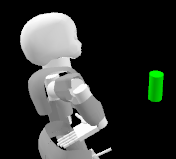
\includegraphics[width=4cm]{./fig_cha3/1_ini.png}}
  \subfloat[\scriptsize{Initial pose 2}] {\label{fig:reachableModelPos}  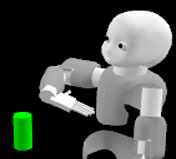
\includegraphics[width=4cm]{./fig_cha3/2_iniss.png}}
  \subfloat[\scriptsize{Initial pose 3}]  {\label{fig:reachableSamplesPos}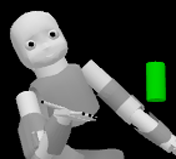
\includegraphics[width=4cm]{./fig_cha3/aa.png}}

  \vspace{0.02in}
  \subfloat[\scriptsize{Final grasp 1}] {\label{fig:reachableSamplesPos}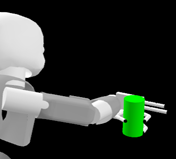
\includegraphics[width=4cm]{./fig_cha3/1_finalss.png}}
  \subfloat[\scriptsize{Final grasp 2}] {\label{fig:reachableModelPos}  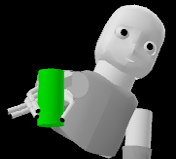
\includegraphics[width=4cm]{./fig_cha3/2_finalss.png}}
  \subfloat[\scriptsize{Final grasp 3}]  {\label{fig:reachableSamplesPos}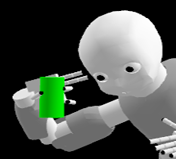
\includegraphics[width=4cm]{./fig_cha3/3_final_2ss.png}}

  \vspace{0.2in}
  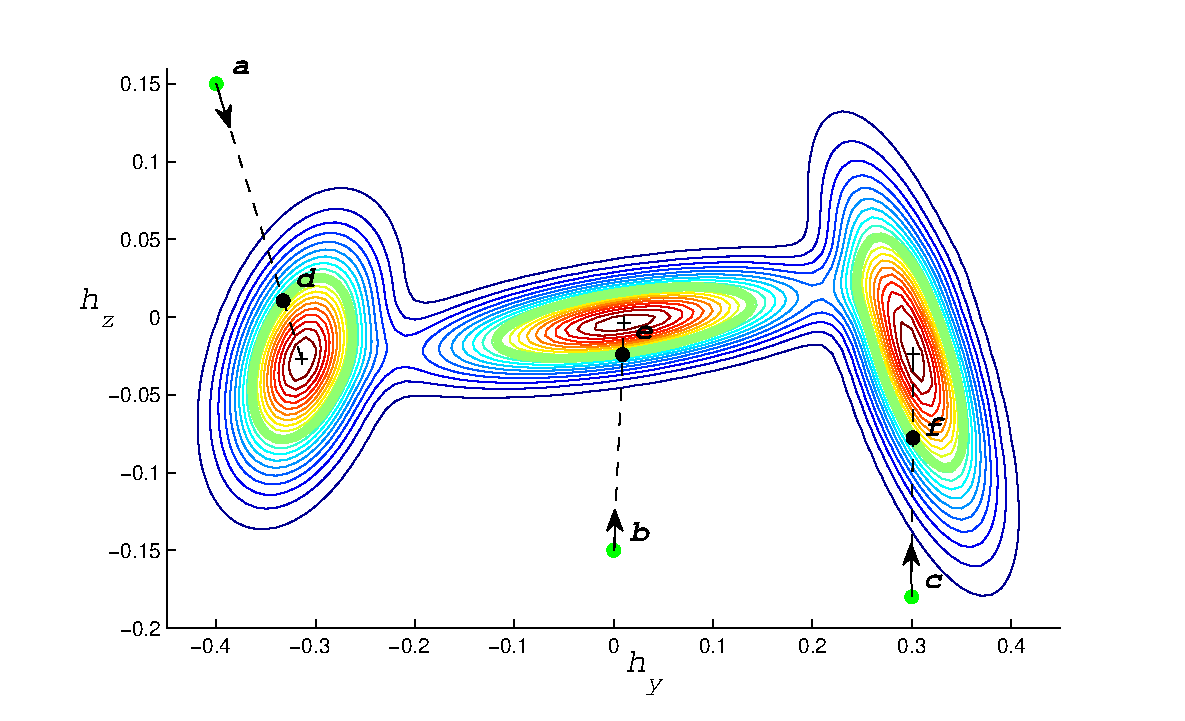
\includegraphics[width=14cm]{./fig_cha3/contour2-3_4.eps}
  \caption{\scriptsize{
  Two-dimensional illustration of the learned model. $h_y$ and $h_z$ correspond to the hand position along the y and z axis of the object reference frame. a, b and c are the initial query points, while d, e and f are their corresponding computed grasps.
  Green dots correspond to initial query inputs  {\bf {\em q}}, black dots correspond to found feasible query inputs {\bf {\em q}}$^*$, contours correspond to parts of the space with constant likelihood, and the thick green contours correspond to threshold values $\eta$ = exp(-$\frac{1}{2}\sigma^2$) of each Gaussian, where $\sigma = 1$ standard deviations.
  The initial finger joint angles in a,b,c are all set to zero. After each feasible query point is found, GMR is used to predict the finger configuration to get the final grasp d,e,f. }
}
    \label{contour}
\end{figure}


\begin{figure}
  \centering
    \subfloat[\scriptsize{Initial pose 1}]  {\label{fig:reachableSamplesPos}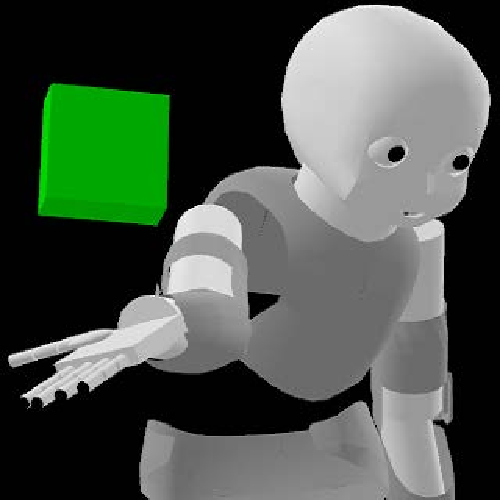
\includegraphics[width=5cm]{./fig_cha3/cuboid_1_i.pdf}}
    \subfloat[\scriptsize{Initial pose 2}] {\label{fig:reachableModelPos}  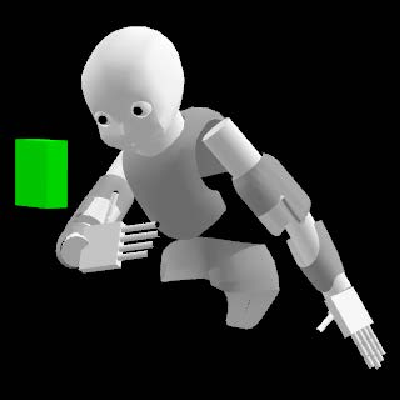
\includegraphics[width=5cm]{./fig_cha3/cuboid_2_i.pdf}}
    \subfloat[\scriptsize{Initial pose 3}] {\label{fig:reachableModelPos}  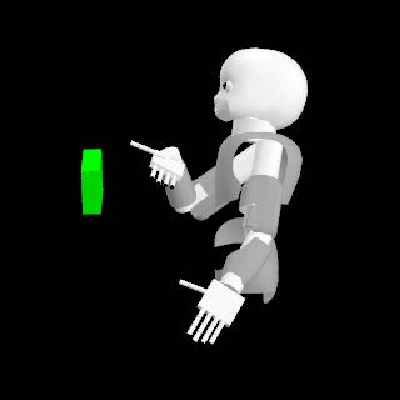
\includegraphics[width=5cm]{./fig_cha3/cuboid_3_i.pdf}}

    %\vspace{0.05in}

    \subfloat[\scriptsize{Final grasp 1}] {\label{fig:reachableModelPos}  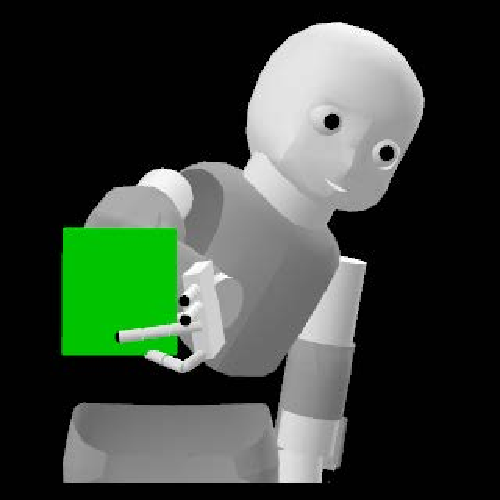
\includegraphics[width=5cm]{./fig_cha3/cuboid_1_f.pdf}}
    \subfloat[\scriptsize{Final grasp 2}]  {\label{fig:reachableSamplesPos}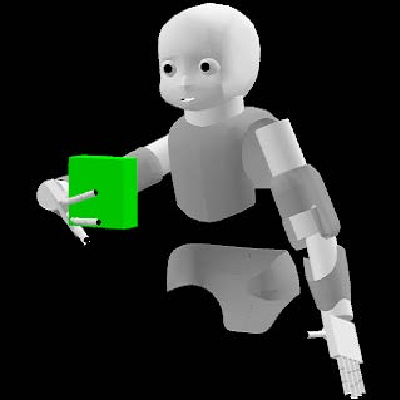
\includegraphics[width=5cm]{./fig_cha3/cuboid_2_f.pdf}}
    \subfloat[\scriptsize{Final grasp 3}]  {\label{fig:reachableSamplesPos}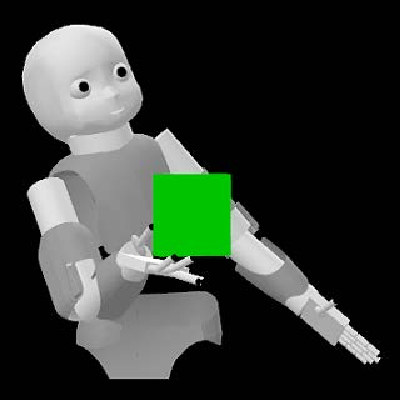
\includegraphics[width=5cm]{./fig_cha3/cuboid_3_f.pdf}}

  \caption{\scriptsize{Examples of the iCub hand grasping a cuboid. The first row (a,b,c) shows the initial postures and the second row (d,e,f) shows the corresponding final grasps.}
}
    \label{icub_cuboid}
\end{figure}

To test the computation time we generated 3000 random initial query points for each grasping task. The initial query points are placed at different distances away from the object surface, varying between 3$cm$ to 50$cm$, and the hand orientation is random. The initial finger configuration is not taken into account in finding the feasible region and hence it is set to the robot hand starting values. The computation time and experimental details are shown in Table~\ref{result}. The computation is done by Matlab on a machine with a 2.8GHz processor and a 4GB RAM.

Table~\ref{result} also shows the success rate of generated grasps with the iCub and the Barrett hand. A grasp is considered to be successful if it satisfies the force-closure criterion, is feasible for the hand kinematics and is not in collision with the object (see Section~\ref{cha3:sec2:demonstration}). When executing the obtained grasp, the fingers will continue to clutch until contact is made; if they contact the object surface before reaching the expected finger configuration, they will halt to avoid penetration.
All the results shown in Figure.~\ref{contour},~\ref{icub_cuboid},~\ref{barrett} are good grasps.

As can be seen from Table~\ref{result}, the success rate depends on the dimensions of the grasp space and the surface geometry of the target objects. Grasps in lower degrees of freedom (the Barrett hand) have higher success rates than those in higher degrees of freedom (the iCub hand). This suggests that the higher dimension grasp space is more complex than the lower dimension grasp space and needs more data to represent the full complexity. On the other hand, objects with smooth surfaces have a success rate around 90\%. Objects with a couple of prominences have success rates over 85\% as the configuration space of grasping is discontinuous. In the Barrett hand and aeroplane model task, the failed grasps are concentrated on two places: the thin edges of the wings and the propeller. Grasping these places requires high accuracy and more training data on these parts would be needed.
%On the other hand, objects with smooth surface have a high rate of success. Objects with a couple of prominence have success rate about 85\% as the configuration space of grasping is discontinue. In the Barrett hand and airplane model task, the failure grasps are concentrated on two places: the thin edges of the wings and the propeller. Grasping these two places require high accuracy and this is not the main concern of this paper.

To compare with the training data, we compute the grasp quality of the results with the same metrics we used in data generation. The mean of the grasp quality of the training set and the result set are similar, though the result set has a slightly higher value in most of cases. We are able to find some grasps of higher quality than all grasps in the training set (Figure~\ref{near}). This shows that GMM is able to model and generalize the high dimensional grasp space, especially for objects with smooth surfaces.

% For the iCub hand, 612 different feasible grasps of a cylindrical object are obtained by the optimization~\citep{sahar2012}. The learned GMM model has 40 Gaussian components, determined by BIC, and each Gaussian has 14 dimensions: hand position (3D), hand orientation (3D), finger joint angles (8D).



\begin{figure}
  \centering
   \subfloat[\scriptsize{Best grasp found}]  {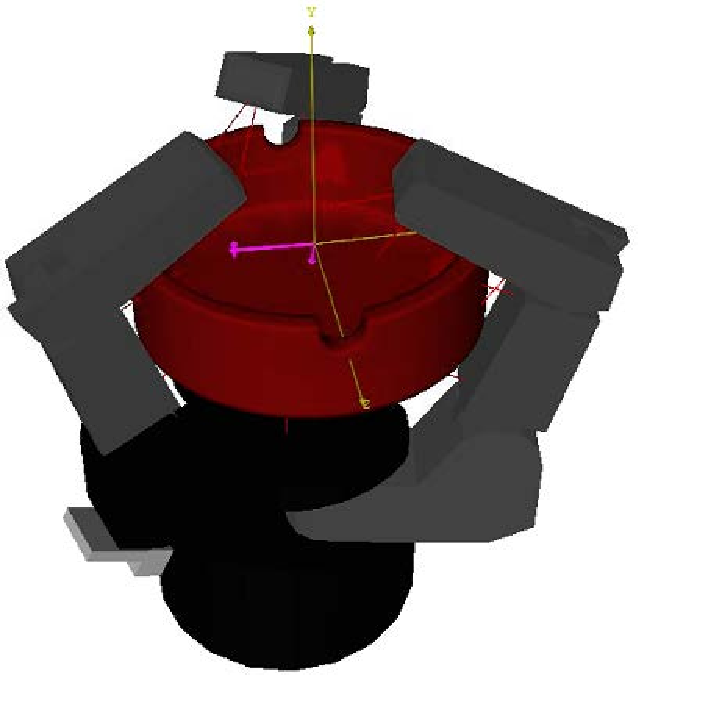
\includegraphics[width=3cm]{./fig_cha3/ash_near1.pdf}}
   \subfloat[\scriptsize{Neighbor grasp of (a)}] {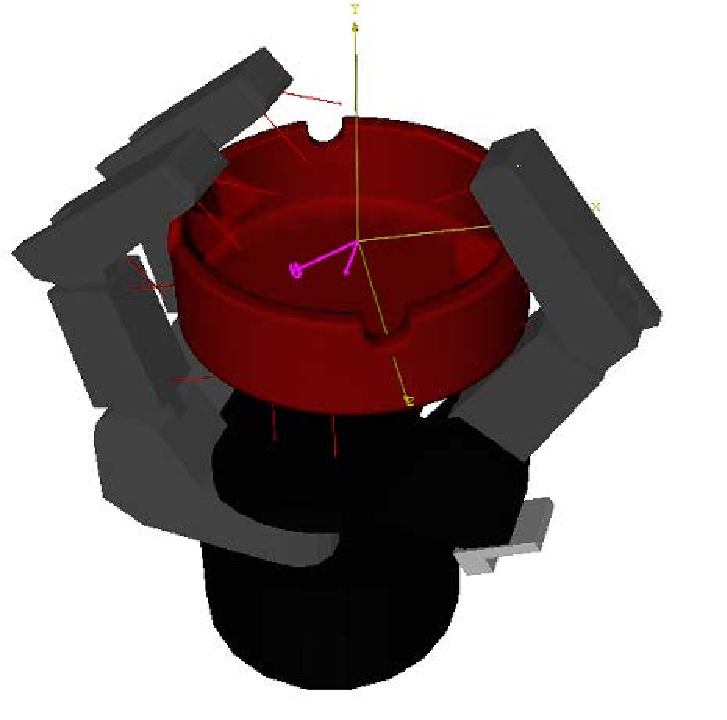
\includegraphics[width=3cm]{./fig_cha3/ash_near2.pdf}}
   \subfloat[\scriptsize{Best grasp found}] {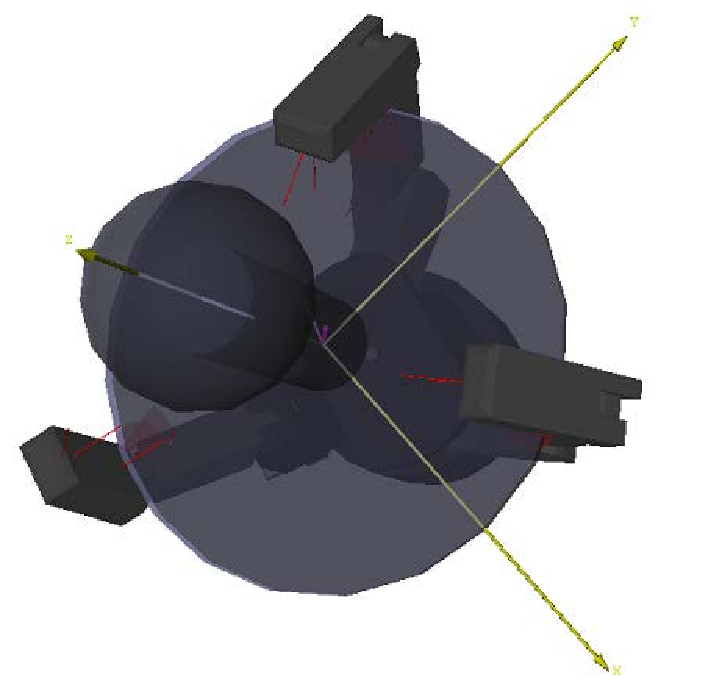
\includegraphics[width=3cm]{./fig_cha3/joy_near1.pdf}}
   \subfloat[\scriptsize{Neighbor grasp of (c)}] {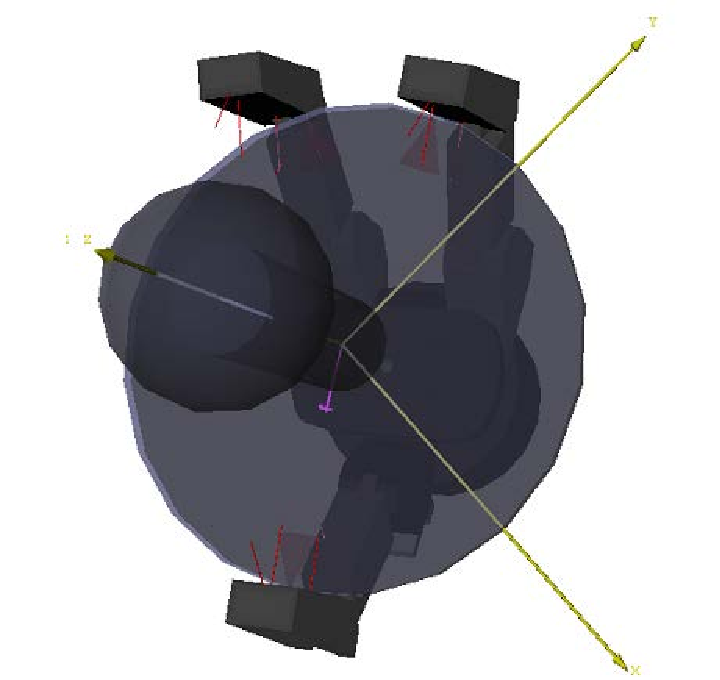
\includegraphics[width=3cm]{./fig_cha3/joy_near2.pdf}}

 \caption{\scriptsize{(a) The best grasp found for the Barrett hand and the ashtray. Grasp Quality is 0.16. (b) The nearest grasp of (a) in the training set. Note the gap between the finger and the object. Grasp Quality is 0.027. (c) The best grasp found for the Barrett hand and the joystick. Grasp Quality is 0.19. (d) The nearest grasp of (b) in the training set. Quality is 0.03 }
}
    \label{near}
\end{figure}


\begin{table*}
\renewcommand{\arraystretch}{1.5}
    \caption{Average computation time for generating new grasps for the iCub hand and the Barrett hand.}
    \hspace{-1.5cm}
    \begin{tabular}{|>{\centering\arraybackslash}p{3cm}|>{\centering\arraybackslash}p{1.2cm}|>{\centering\arraybackslash}p{1.7cm}|>{\centering\arraybackslash}p{1.2cm}|>{\centering\arraybackslash}p{1.5cm}|>{\centering\arraybackslash}p{1.5cm}|>{\centering\arraybackslash}p{1.7cm}|>{\centering\arraybackslash}p{1.7cm}|>{\centering\arraybackslash}p{0.9cm}|}%{ | c | c | c | c | c | c | c | c |p{1cm} |}
    \hline
    Robot/Object & Number of training data & Average Grasp Quality(train)& Number of Gaussians& Force-Closure Grasp Found & Average Grasp Quality(result)& Mean of Computation Time($msec$) & Variance ($msec$)   \\ \hline
    iCub/Cylinder       & 621   & 0.0965& 40    & 90\%  & 0.1008    & 9.1   & 0.0001 \\ \hline
    iCub/Cuboid         & 532   & 0.1317& 40    & 89\%  & 0.1224    & 9.4   & 0.0007 \\ \hline
    Barrett/Ashtray     & 1560  & 0.0975& 15    & 100\% & 0.1644    & 4.3   & 0.0001 \\ \hline
    Barrett/Shoe        & 629   & 0.0019& 25    & 99\%  & 0.0034    & 6.9   & 0.0001 \\ \hline
    Barrett/Joystick    & 1500  & 0.0061& 20    & 98\%  & 0.0064    & 5.9   & 0.0002 \\ \hline
    Barrett/Plane       & 1374  & 0.0002& 55    & 85\%  & 0.0003    & 15.1  & 0.0003 \\ \hline

    \end{tabular}

    \label{result}

\end{table*}


\begin{figure*}
  \centering

    \subfloat[\scriptsize{Initial pose 1}]  {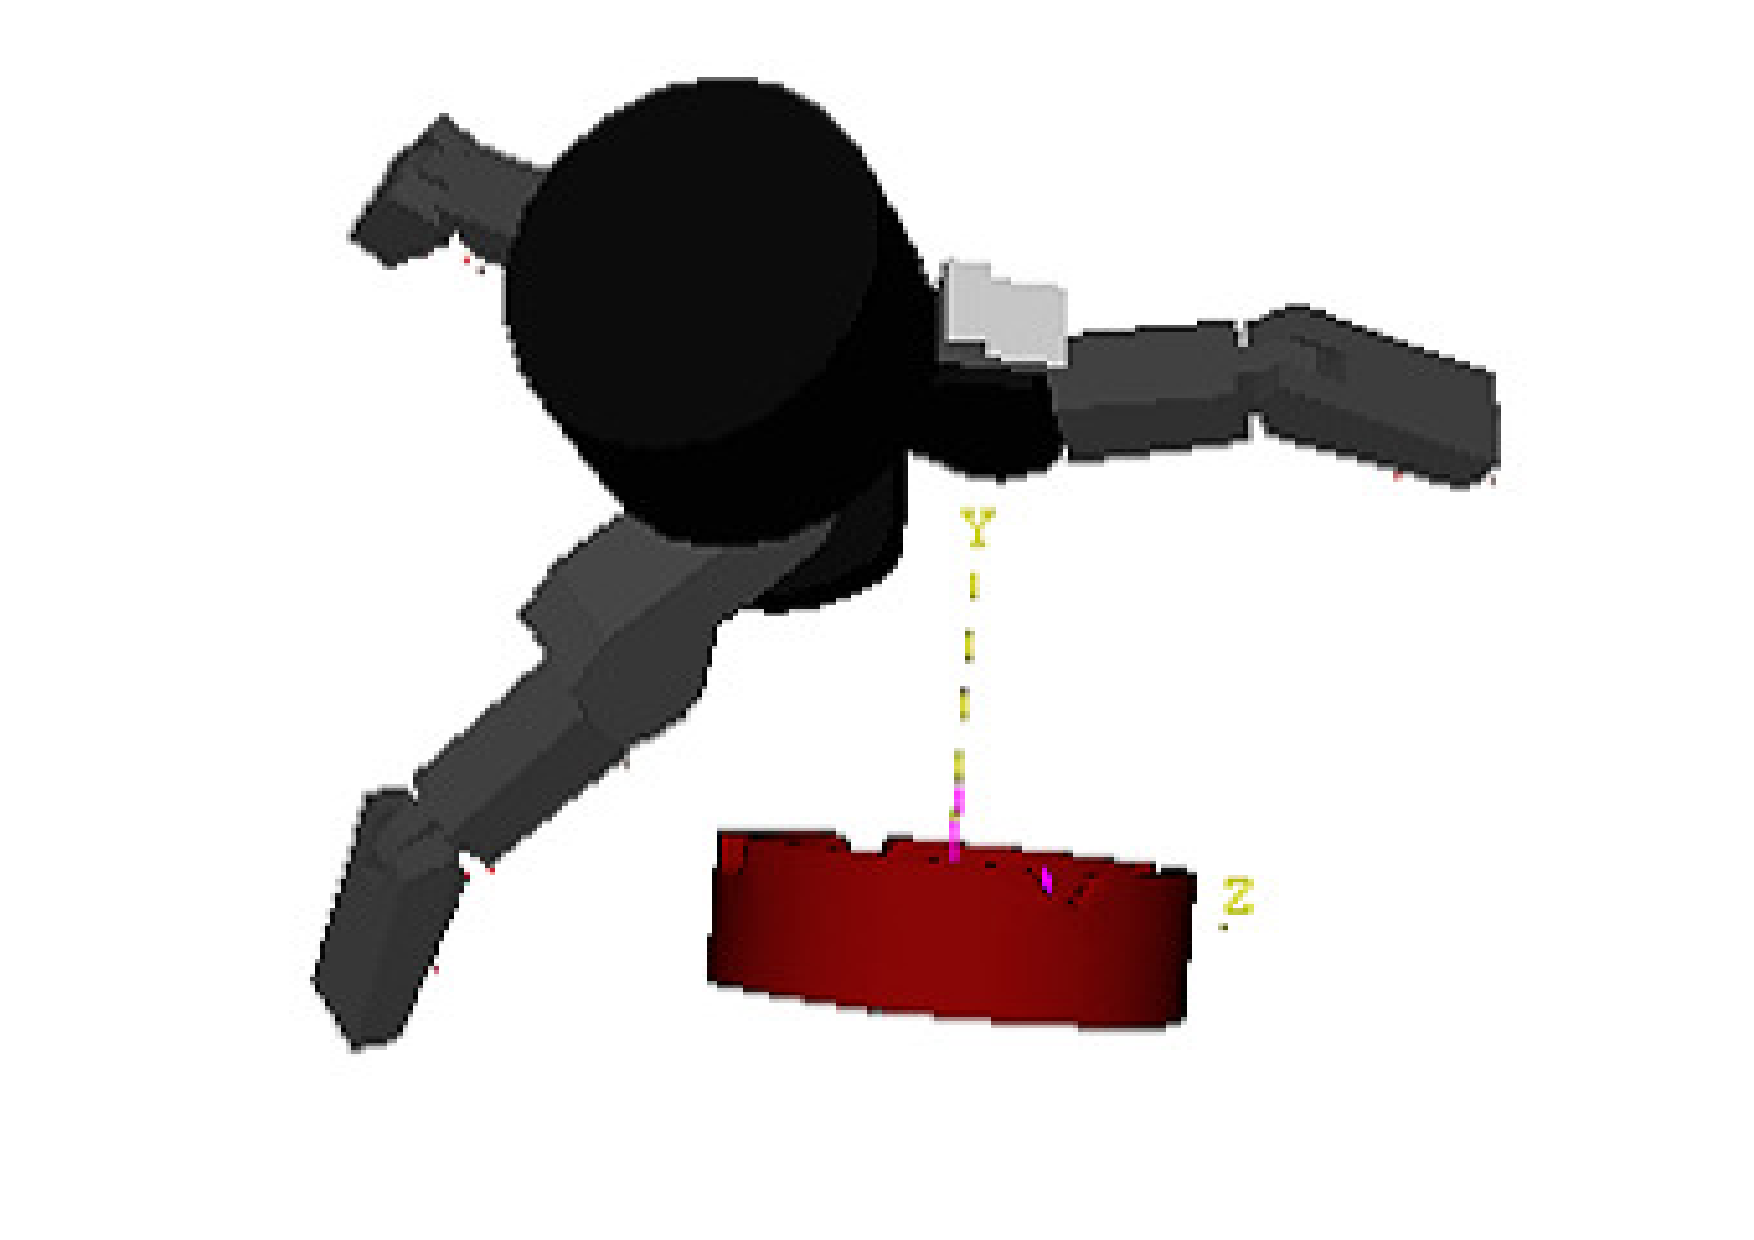
\includegraphics[width=4cm]{./fig_cha3/bar_i_1.pdf}}
    \subfloat[\scriptsize{Initial pose 2}] { 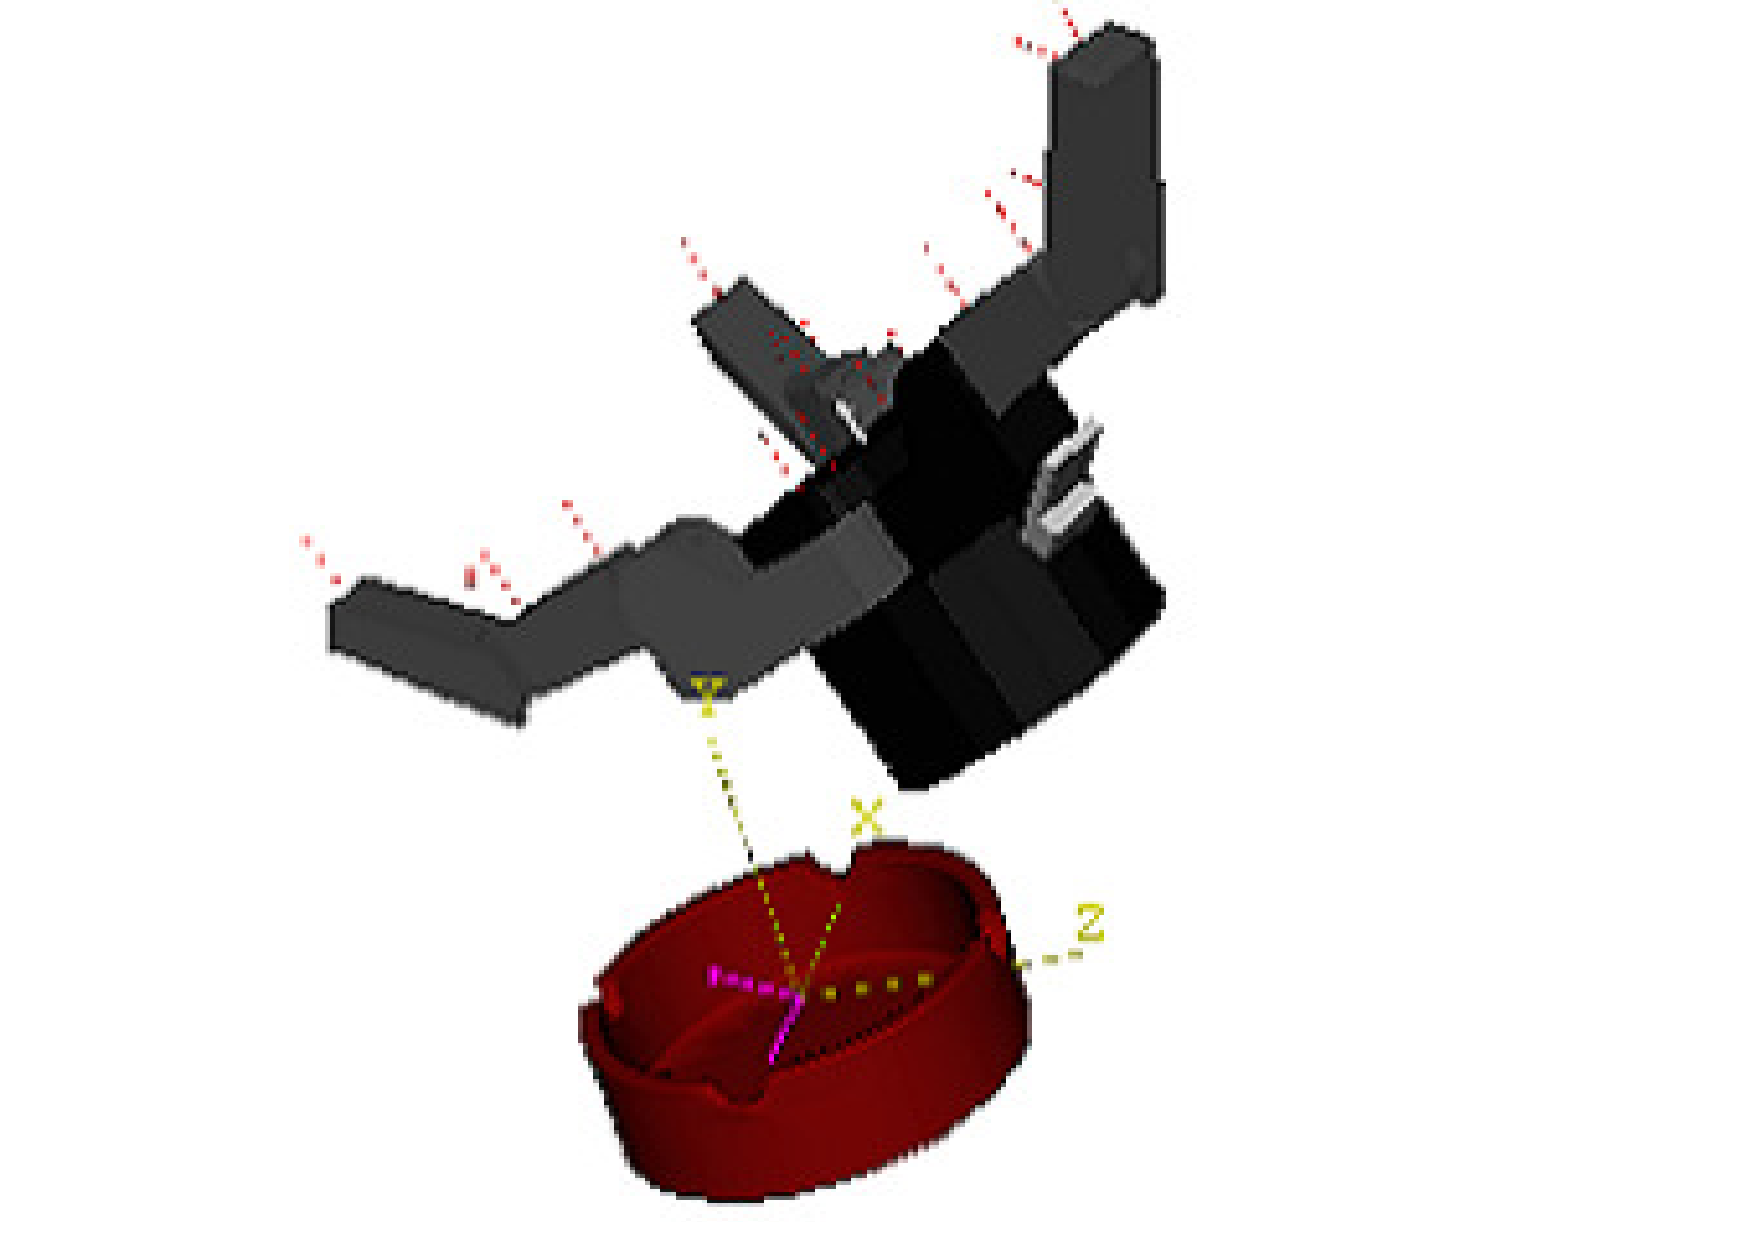
\includegraphics[width=4cm]{./fig_cha3/bar_i_2.pdf}}
    \subfloat[\scriptsize{Initial pose 3}] { 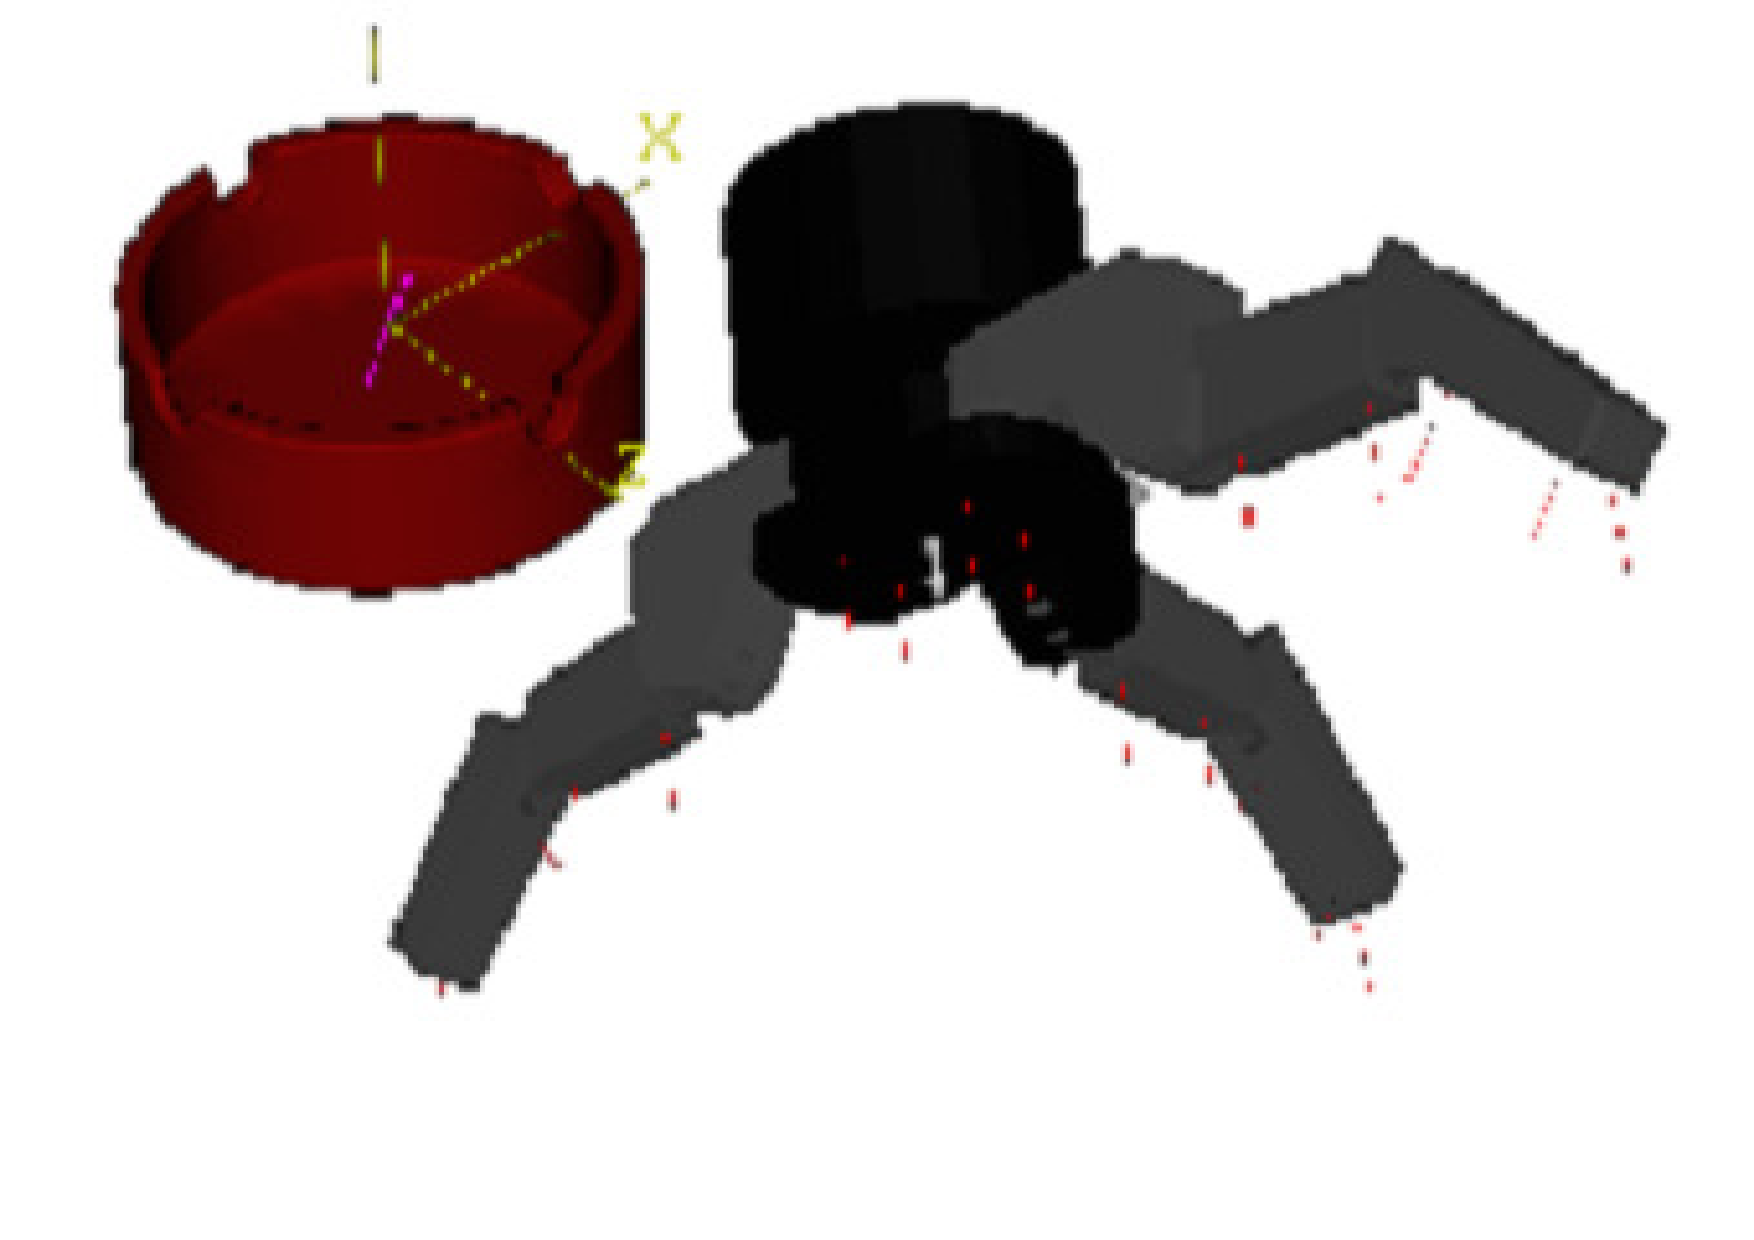
\includegraphics[width=4cm]{./fig_cha3/bar_i_3.pdf}}
    \vspace{0.3cm}
    \subfloat[\scriptsize{Final grasp 1}] {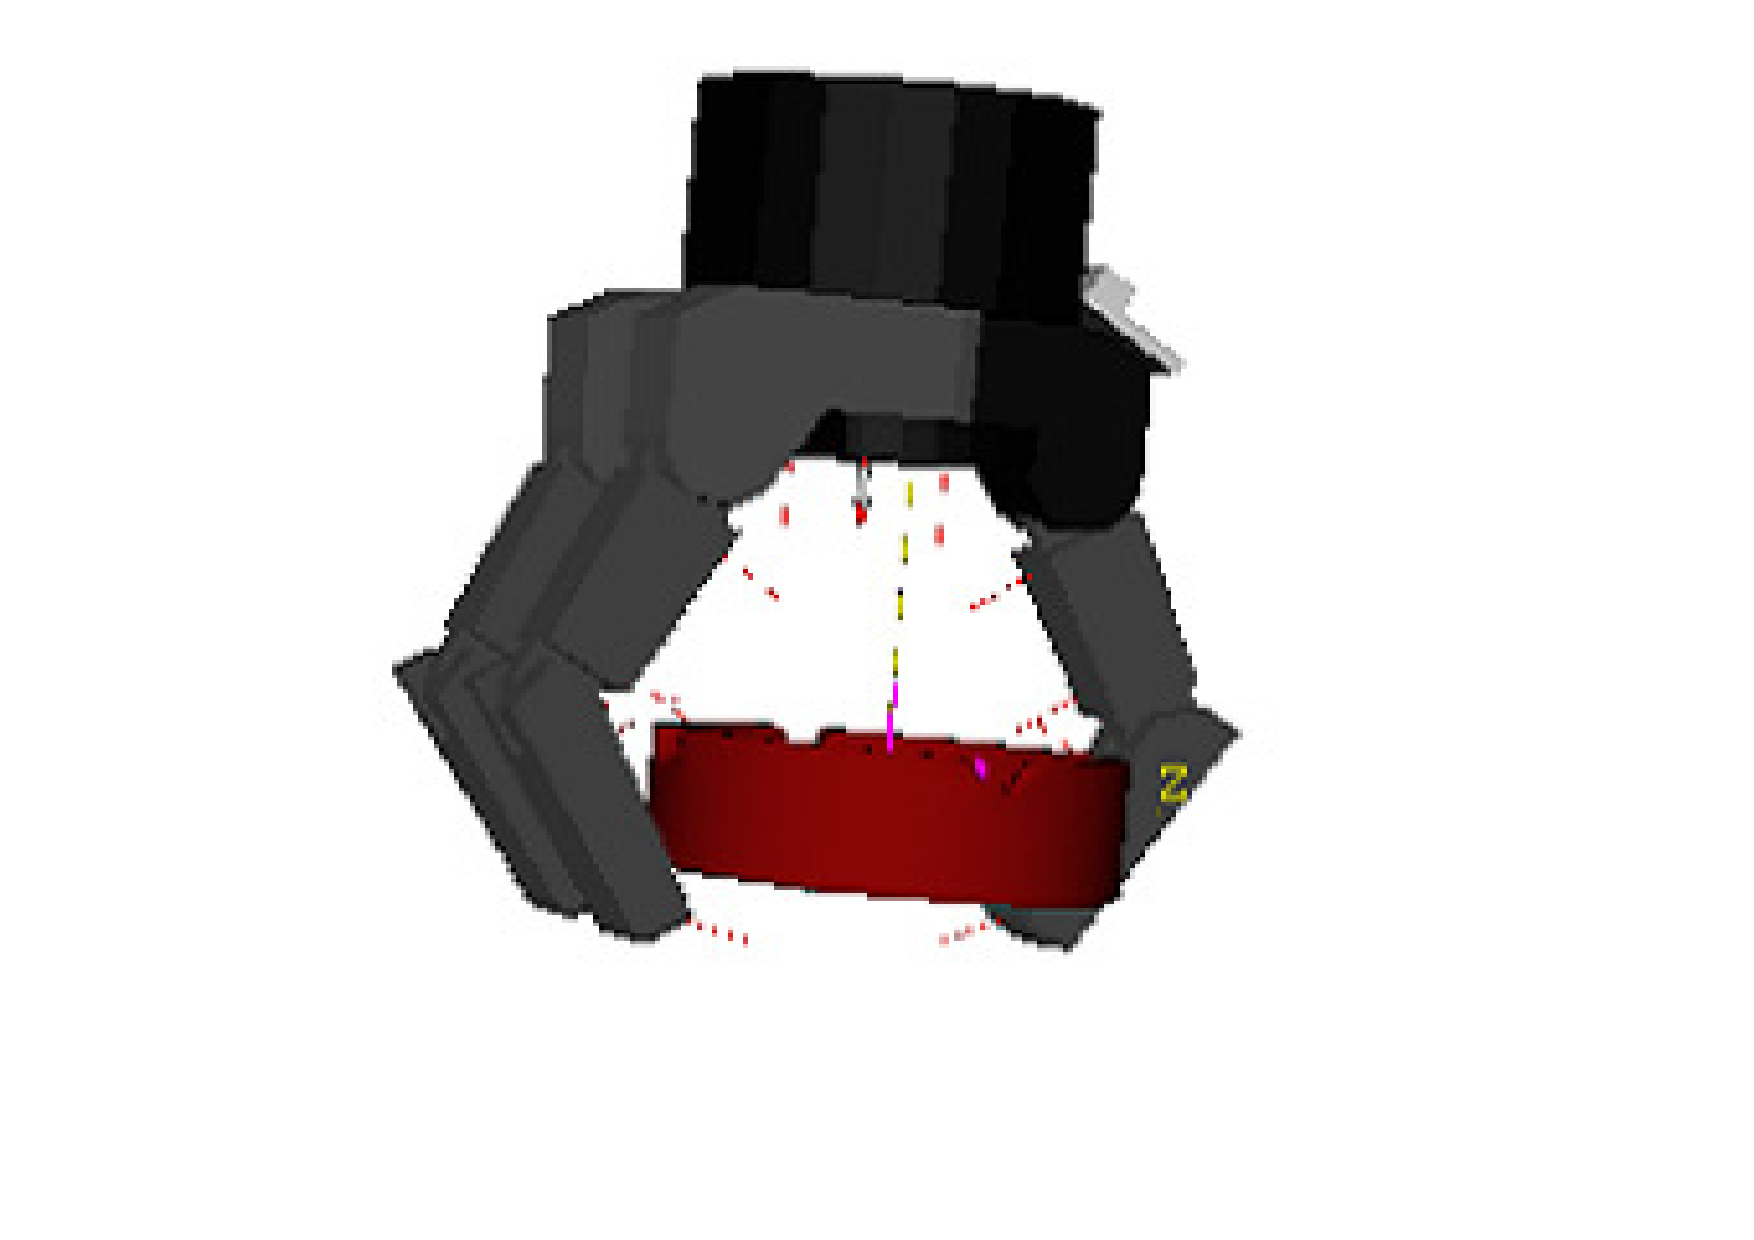
\includegraphics[width=4cm]{./fig_cha3/bar_f_1.pdf}}
    \subfloat[\scriptsize{Final grasp 2}]  {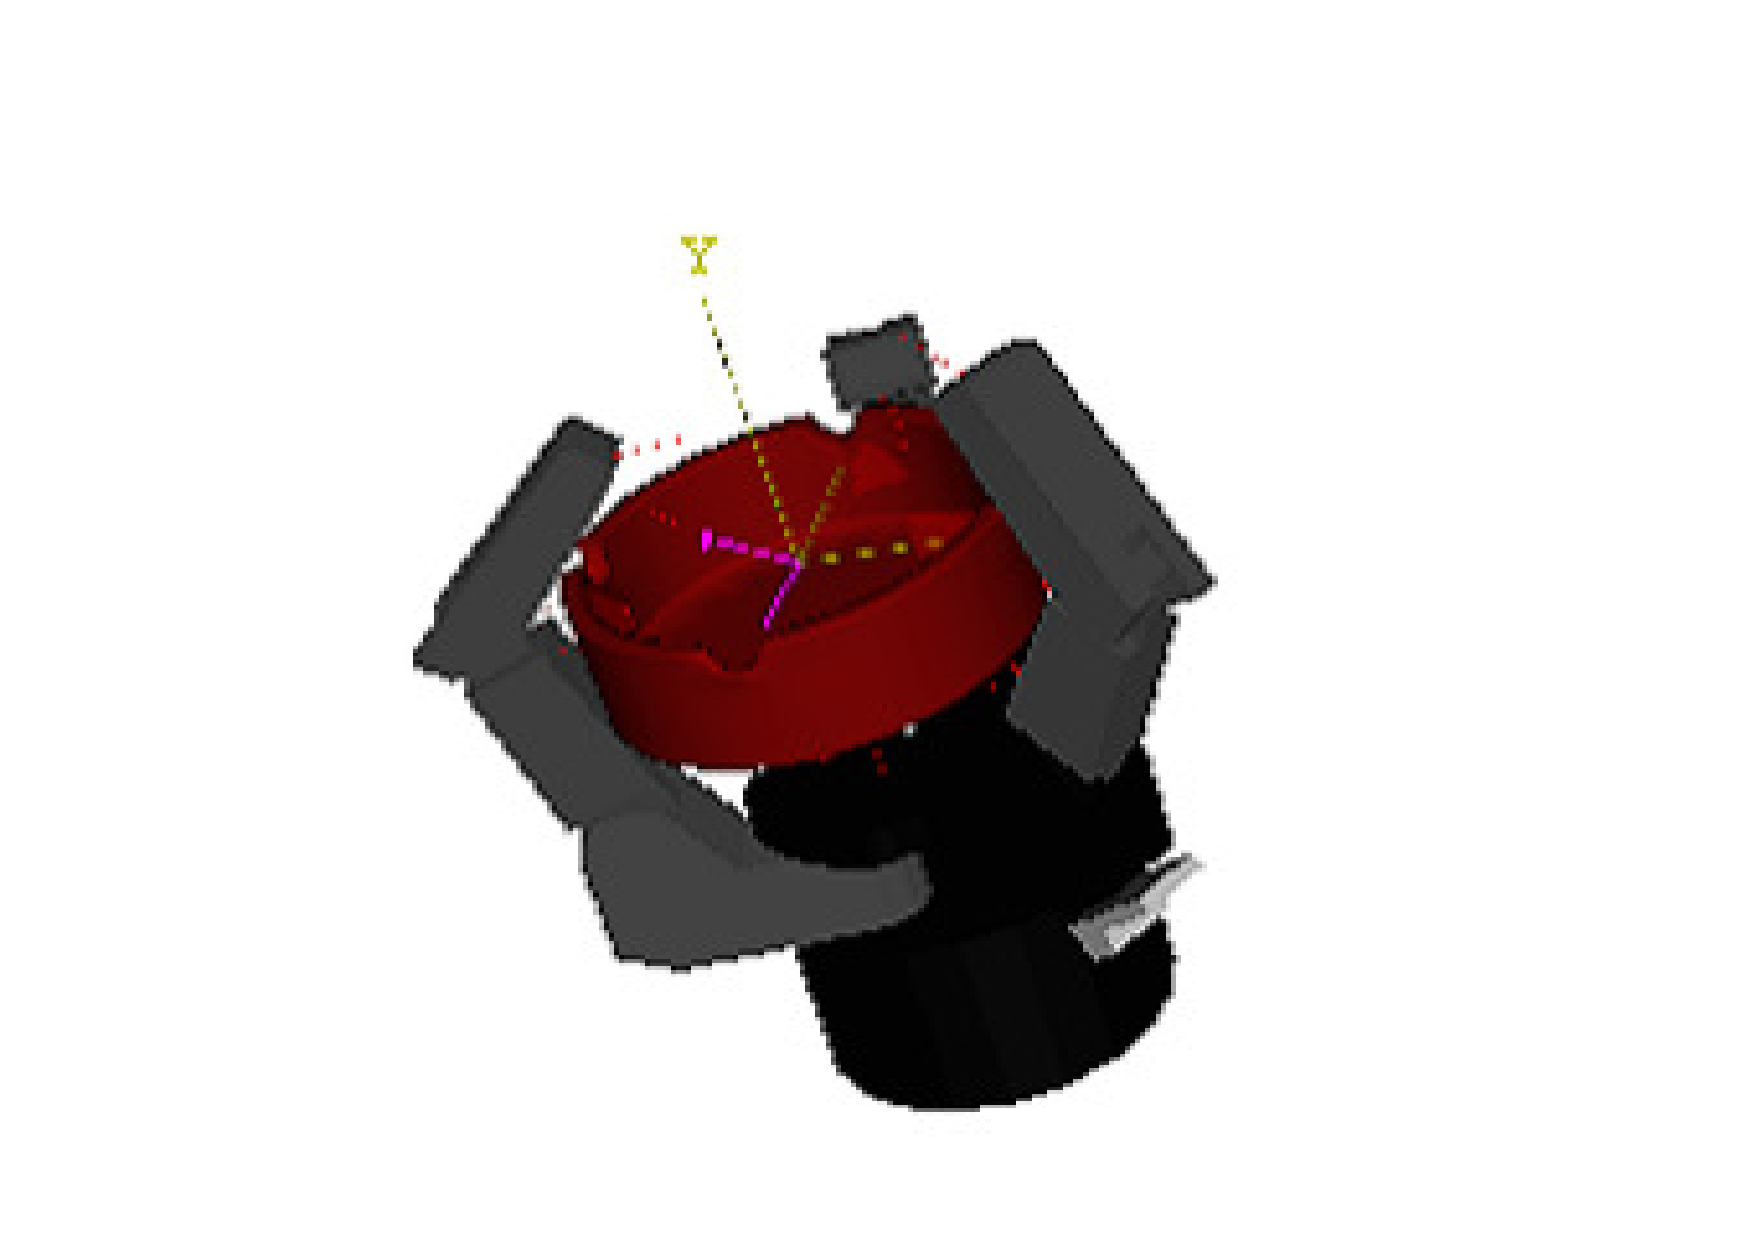
\includegraphics[width=4cm]{./fig_cha3/bar_f_2.pdf}}
    \subfloat[\scriptsize{Final grasp 3}]  {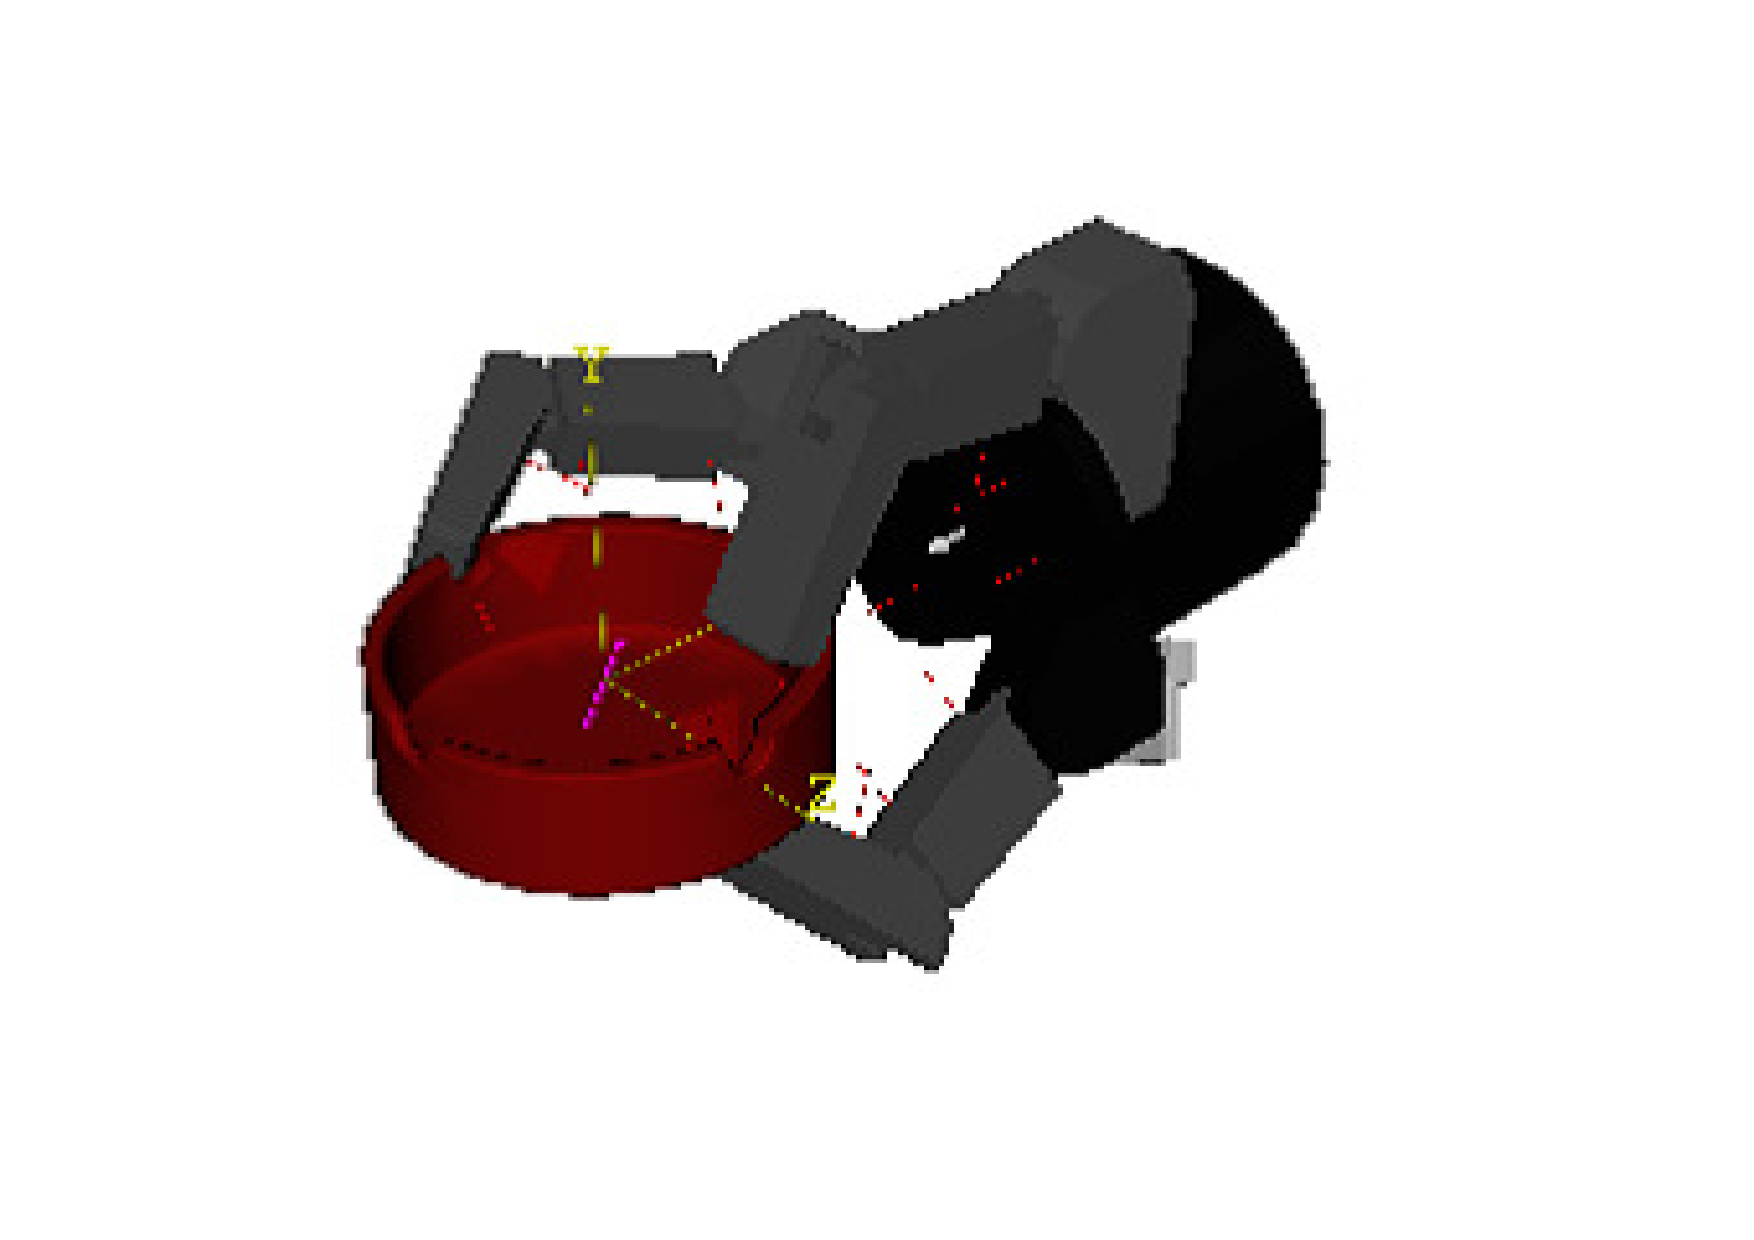
\includegraphics[width=4cm]{./fig_cha3/bar_f_3.pdf}}
    \vspace{0.3cm}
    \subfloat[\scriptsize{Initial pose 4}]  {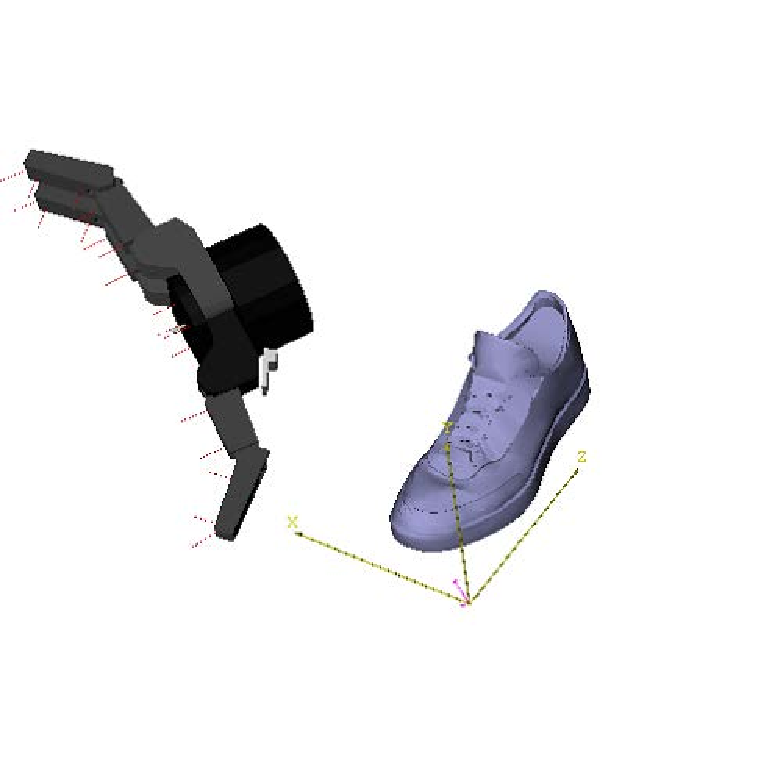
\includegraphics[width=4cm]{./fig_cha3/shoe_1i.pdf}}
    \subfloat[\scriptsize{Initial pose 5}] {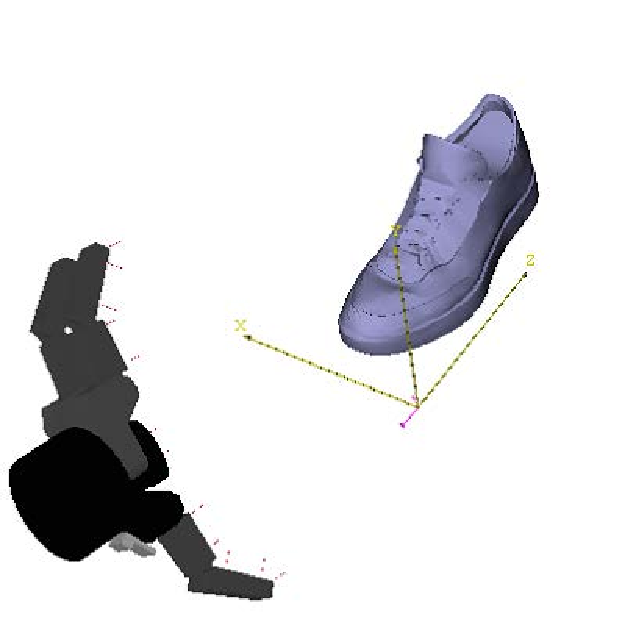
\includegraphics[width=4cm]{./fig_cha3/shoe_2i.pdf}}
    \subfloat[\scriptsize{Initial pose 6}]  {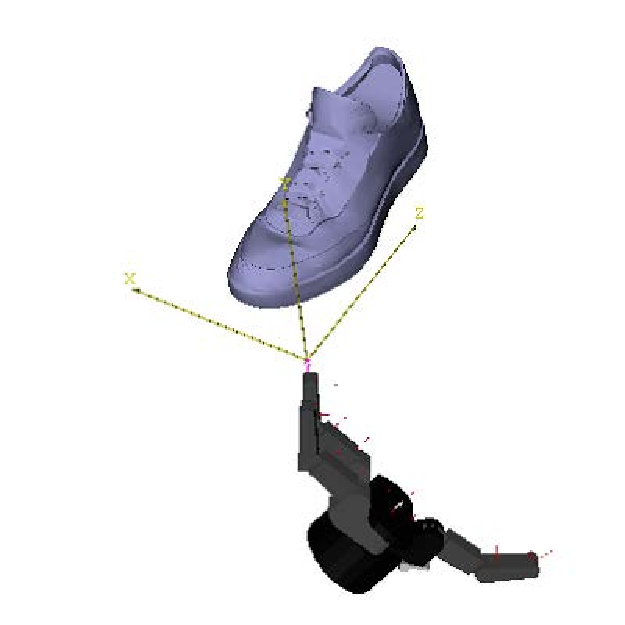
\includegraphics[width=4cm]{./fig_cha3/shoe_3i.pdf}}
    \vspace{0.3cm}
    \subfloat[\scriptsize{Final grasp 4}] {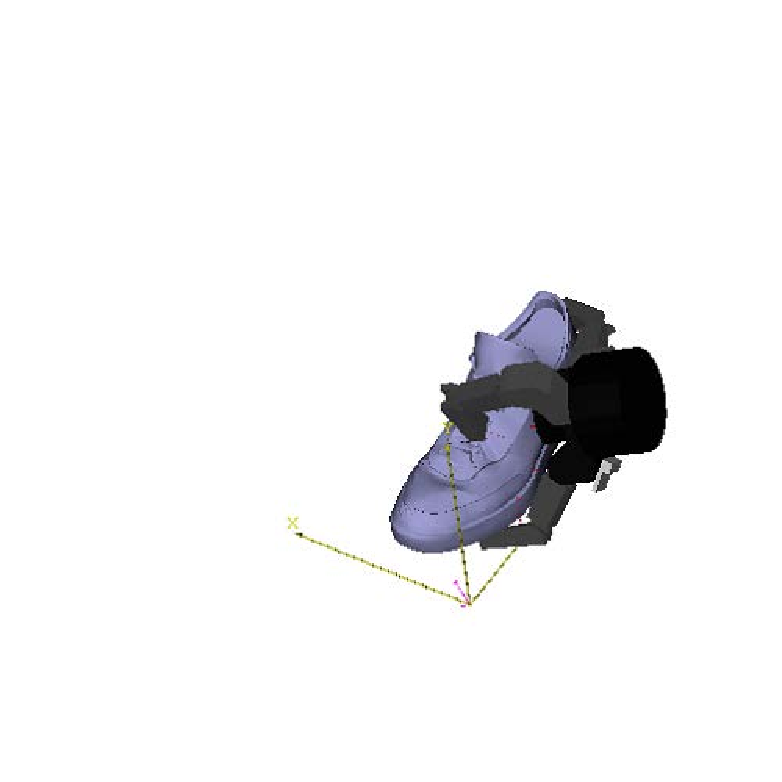
\includegraphics[width=4cm]{./fig_cha3/shoe_1f.pdf}}
    \subfloat[\scriptsize{Final grasp 5}] {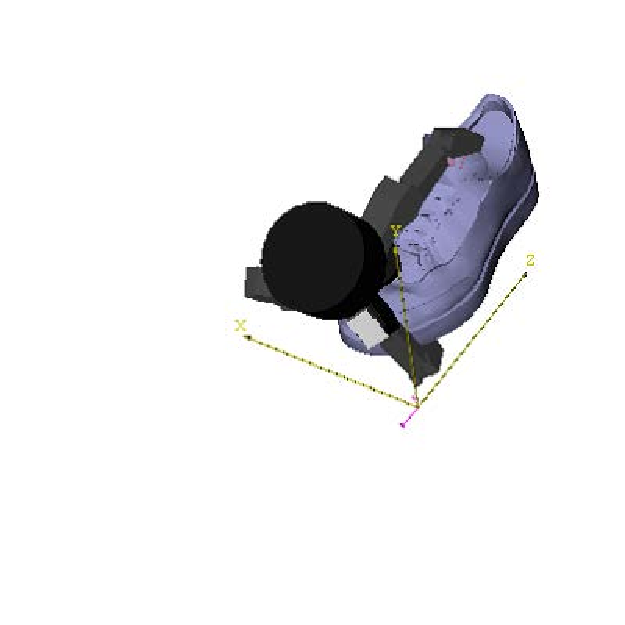
\includegraphics[width=4cm]{./fig_cha3/shoe_2f.pdf}}
    \subfloat[\scriptsize{Final grasp 6}]  {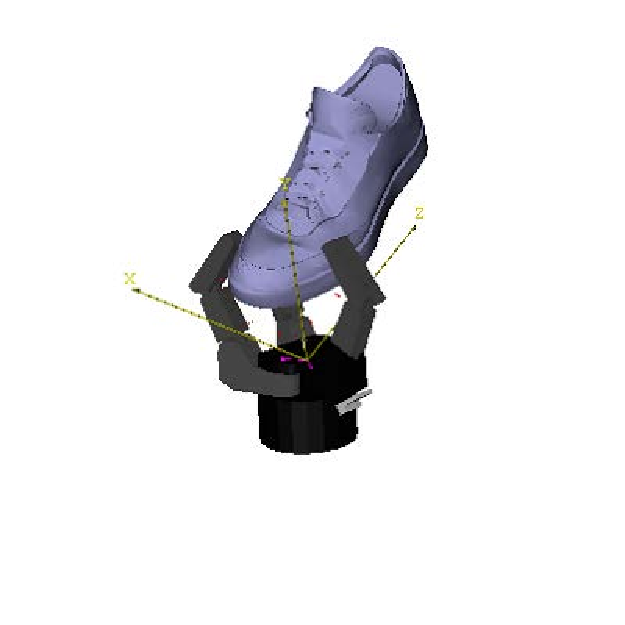
\includegraphics[width=4cm]{./fig_cha3/shoe_3f.pdf}}

  \caption{\scriptsize{Examples of Barrett hand grasping different objects (ashtray, shoe).
 The first and third rows (a,b,c and g,h,i) show the initial postures and the second and forth rows (d,e,f and j,k,l) show the corresponding final grasps.}
}
    \label{barrett}
\end{figure*}

\begin{figure*}
  \centering
    \subfloat[\scriptsize{Initial pose 7}]  {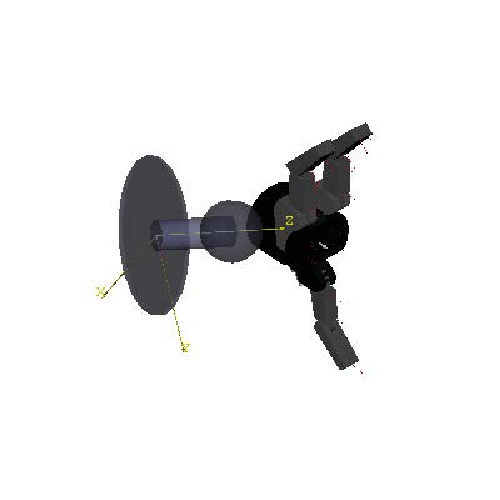
\includegraphics[width=4cm]{./fig_cha3/joy_2_i.pdf}}
    \subfloat[\scriptsize{Initial pose 8}] {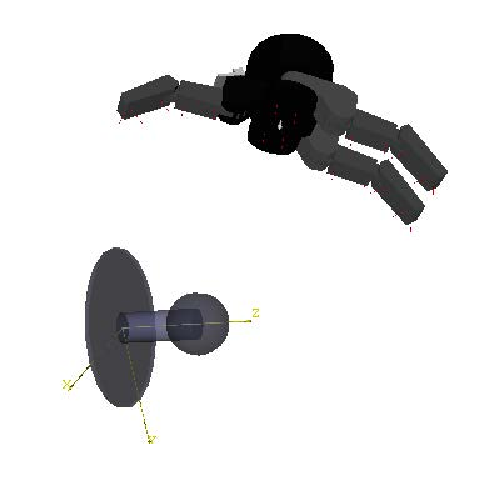
\includegraphics[width=4cm]{./fig_cha3/joy_3_i.pdf}}
    \subfloat[\scriptsize{Initial pose 9}] {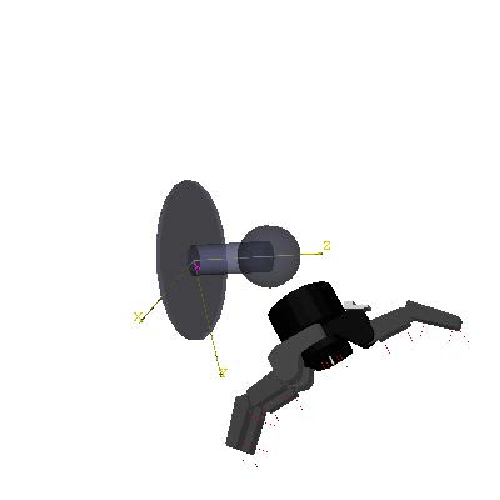
\includegraphics[width=4cm]{./fig_cha3/joy_5_i.pdf}}
    \vspace{0.3cm}
    \subfloat[\scriptsize{Final grasp 7}] {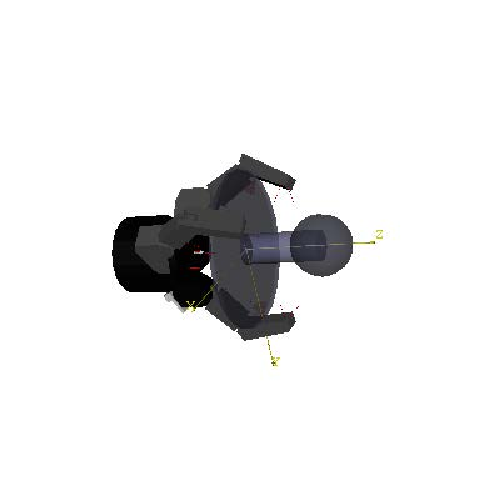
\includegraphics[width=4cm]{./fig_cha3/joy_2_f.pdf}}
    \subfloat[\scriptsize{Final grasp 8}]  {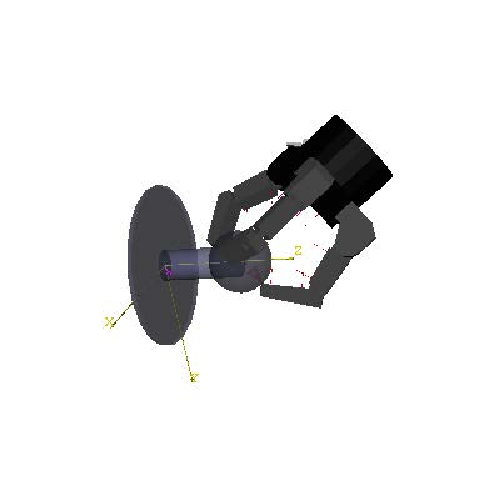
\includegraphics[width=4cm]{./fig_cha3/joy_3_f.pdf}}
    \subfloat[\scriptsize{Final grasp 9}]  {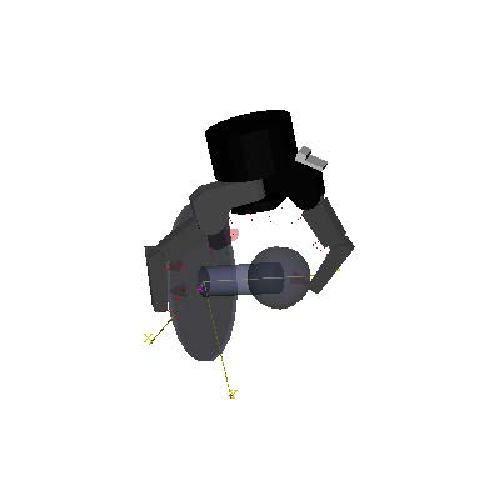
\includegraphics[width=4cm]{./fig_cha3/joy_5_f.pdf}}
    \vspace{0.3cm}
    \subfloat[\scriptsize{Initial pose 10}]  {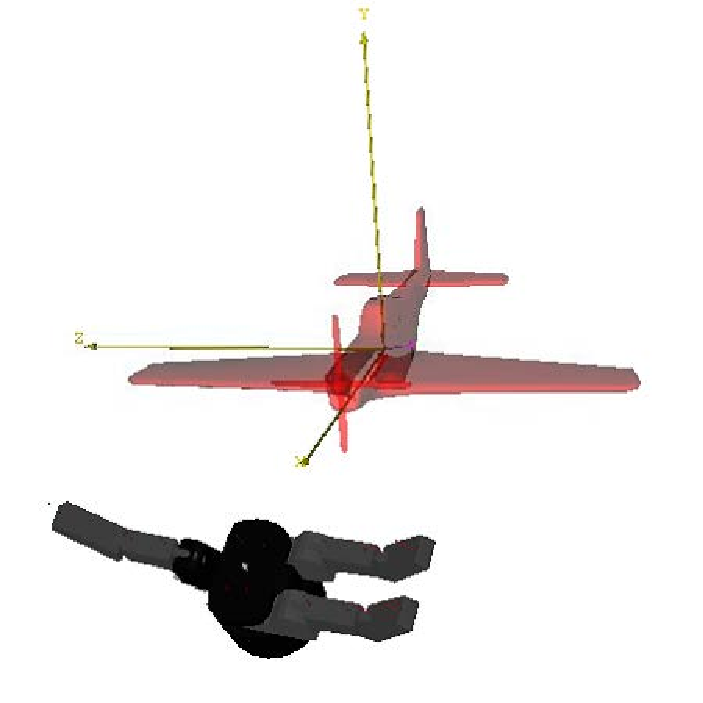
\includegraphics[width=4cm]{./fig_cha3/plane_2i.pdf}}
    \subfloat[\scriptsize{Initial pose 11}] {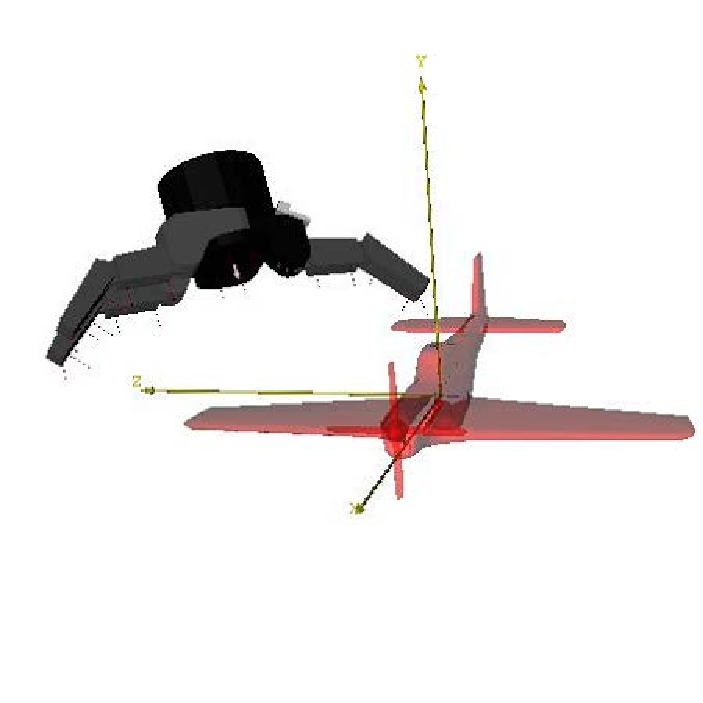
\includegraphics[width=4cm]{./fig_cha3/plane_3i.pdf}}
    \subfloat[\scriptsize{Initial pose 12}] {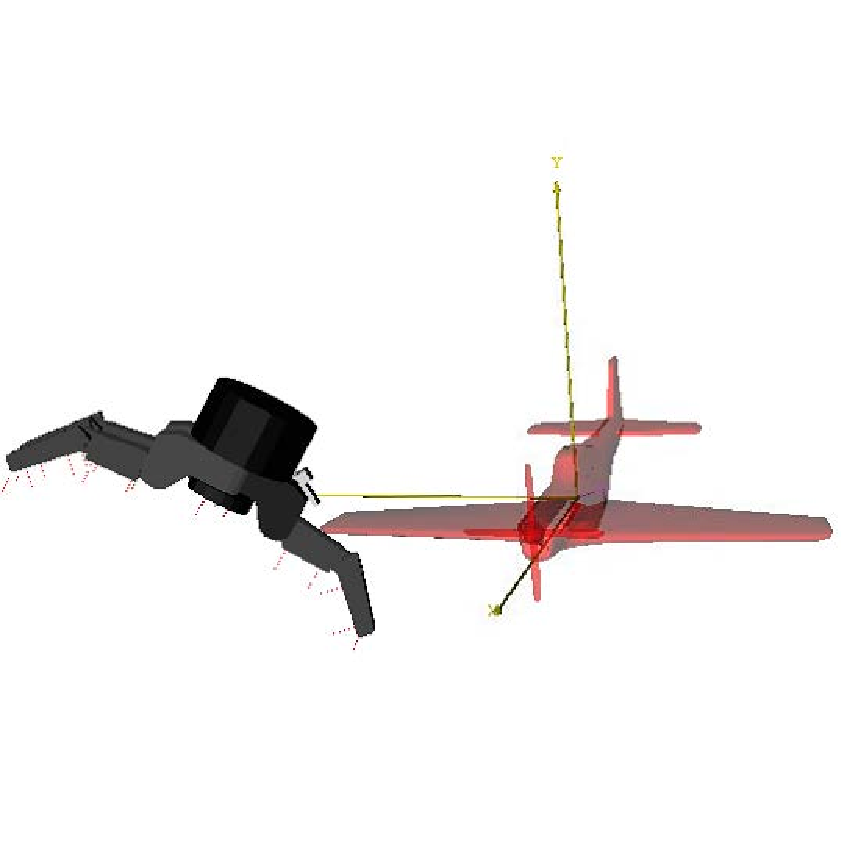
\includegraphics[width=4cm]{./fig_cha3/plane_1i.pdf}}
    \vspace{0.3cm}
    \subfloat[\scriptsize{Final grasp 10}] {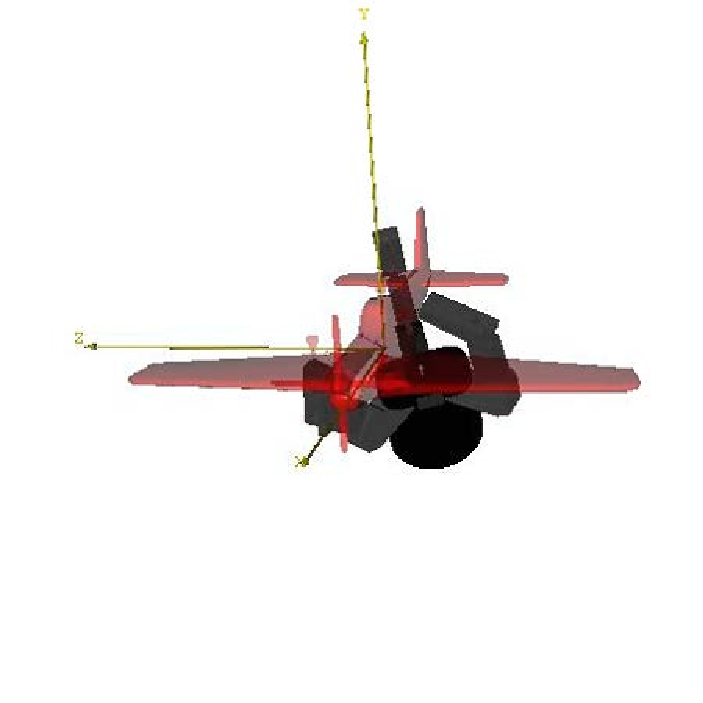
\includegraphics[width=4cm]{./fig_cha3/plane_2f.pdf}}
    \subfloat[\scriptsize{Final grasp 11}]  {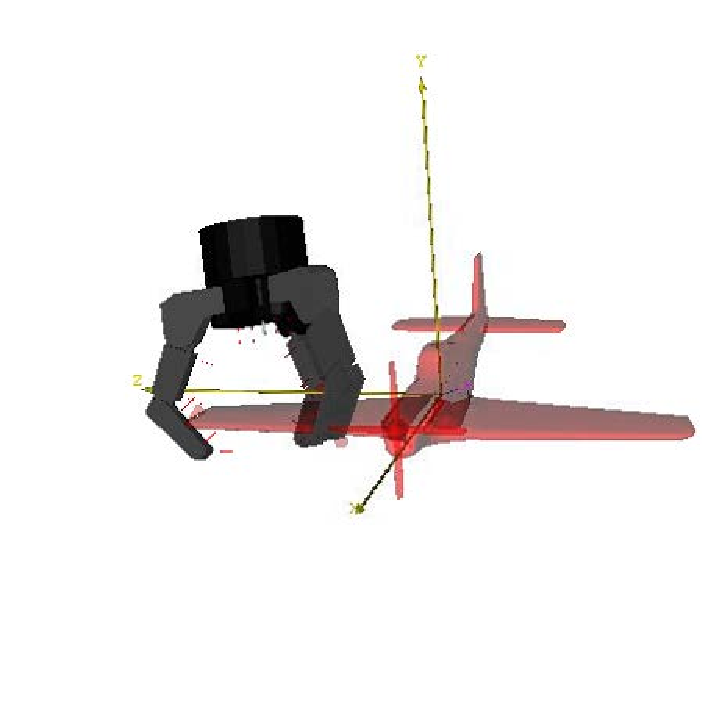
\includegraphics[width=4cm]{./fig_cha3/plane_3f.pdf}}
    \subfloat[\scriptsize{Final grasp 12}]  {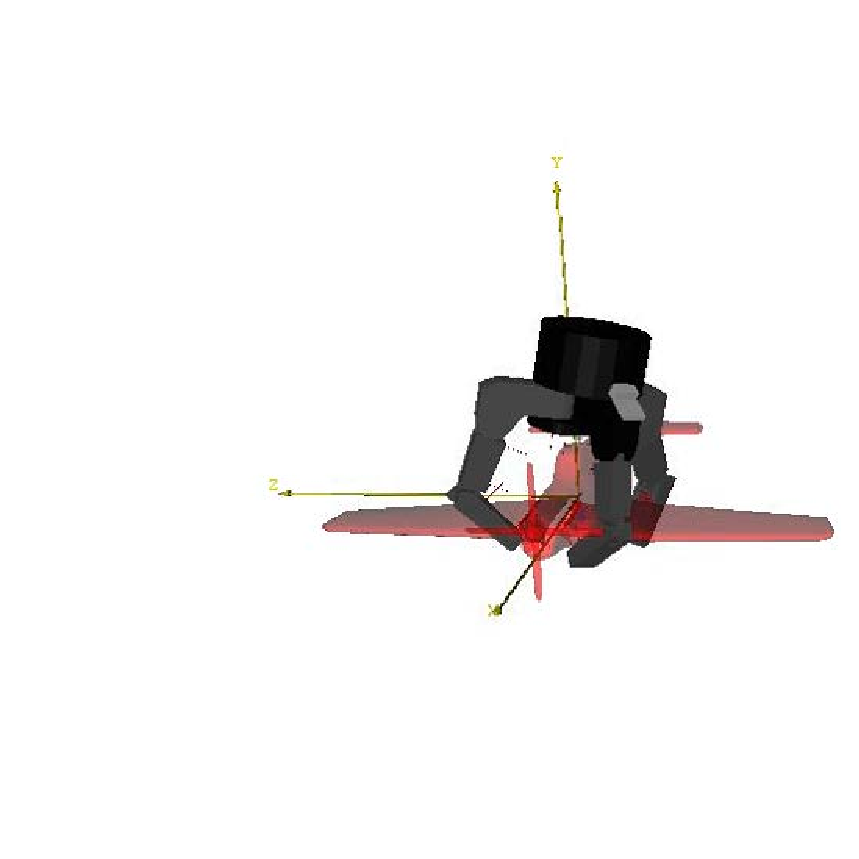
\includegraphics[width=4cm]{./fig_cha3/plane_1f.pdf}}

  \caption{\scriptsize{Examples of Barrett hand grasping different objects (joystick, aeroplane model). The first and third rows (a,b,c and g,h,i) show the initial postures and the second and forth rows (d,e,f and j,k,l) show the corresponding final grasps.}
}
    \label{barrett2}
\end{figure*}



%This approach provides a good estimation of a stable and feasible grasp for the given object and robot hand. In contrast to the common approach of learning from human demonstrations, these grasps are generated solely according to the mechanics of the robot hand. Some resulting grasps are markedly different from  human grasps, especially for the Barrett hand which is very different from the human hand. Our method may therefore out-perform human demonstrations in some contexts by better exploiting differences between human and robot ``physiology''.

To model the actual contact points between the robot hand and the object is difficult in real time because of the high dimensionality of the solution space and the non-linearity of the kinematic constraints. In our method, instead of computing the actual contact point position, we compute the most likely solution using a GMM. Though a certain amount of accuracy is traded off to achieve the real time goal, the overall performance is satisfying. In the experiments listed above, over 90 percent of the testing points find good grasps within a few milliseconds. This method is most efficient for objects with a smooth surface. For complex objects this method can achieve a high success rate of over 85\%. When grasping the parts requiring high precision, additional feedback from visual or tactile sensors is needed for further refinement of the grasp.

This approach requires the object model to be pre-trained. This is to say, we can only plan grasps for familiar objects with this method. It is useful for a robot working in a controlled environment with a limited number of objects, such as in operating theatres. For domestic service robots, however, this is not enough. New objects will continuously come to the house and hence the robot has to be able to grasp novel object shapes. An extension of this method to work on novel objects is discussed in the next two sections.

%The way we project the initial query point to the closest Gaussian component is more conservative.



\section{Grasping novel objects based on familiar parts}
\label{cha3:sec4}
A method to compute grasps for novel objects is in need for domestic service robots. In this chapter we study the problem of generating grasps for un-trained objects in real time.

Objects used in daily life have a variety of shapes. Very often they share similar shape parts, such as sphere, cylinder and box. These shapes repeatedly appear in our daily life, being the object shape or the part of the object shape. Hence we call them``shape primitives''.

To work with un-trained objects, we take the grasping by shape primitives approach~\citep{miller2003automatic}. This approach makes the assumption that all object shapes can be decomposed into a set of primitive shapes where grasps can be planned easily. Based on this assumption, we firstly build a set of GMMs to model the grasp distribution $\left(\Omega_i, i=1,2,...N\right)$ for a set of $N$ chosen shape primitives. When an unseen object is presented, of which the shape can be approximated as a combination of known shape primitives, it's grasp distribution is built by combining the primitives' models. The combined model is then used to quickly generate new grasps.

%\subsection{Combine grasp distribution of shape primitives}
%\label{cha3:sec4:combine}


\subsection{Primitive grasp distribution}
\label{cha3:sec4:pgdistribution}
%\subsubsection{Primitive grasp distribution}
%\label{cha3:sec4:combine:primitivegraspdistribution}
Here we define our shape primitives to be a set of superquadrics. We learn the grasp distributions for a set of superquadrics and use them as the ``primitive grasp distribution''.


\paragraph{Superquadrics} ~\\
%\label{cha3:sec4:combine:primitivegraspdistribution:sq}
Superquadrics are a family of geometric shapes that includes a large variety of shapes we use in daily life, such as cuboid, sphere and cylinder. We choose superquadrics as our shape primitives for three reasons. Firstly, superquadrics and their combinations can be used to represent most of the daily life objects. The wide use of superquadrics in computer graphics and the game industry for modelling object shapes shows its versatility. Secondly, all superquadrics are symmetric to their $x, y, z$ axis. This can reduce the number of testing grasps to 1/8. Thirdly, it's implicit expression is convenient for combining the grasp density, which will be explained in detail in the Section~\ref{cha3:sec4:combine:combining}.

To represent a superquadric we have:

\begin{equation}
r\left(x, y ,z\right) =
\left(\left(\frac{x-x_0}{a_1}\right)^{\frac{2}{\epsilon_2}} +
    \left(\frac{y-y_0}{a_2}\right)^{\frac{2}{\epsilon_2}}\right)^
    {\frac{\epsilon_2}{\epsilon_1}} +
    \left(\frac{z-z_0}{a_3}\right)^\frac{2}{\epsilon_1}
\end{equation}
where $\left(x_0, y_0, z_0\right)$ is the center, $a_1, a_2, a_3$ define the scale in the $x, y, z$ axis respectively, and $\epsilon_1, \epsilon_2$ define the shape of the superquadric.
We use the value of $r$ to measure the relative position of a point $x, y, z$ to the superquadric shape:
\begin{equation}
    r
    \begin{cases}
      <1, & \text{inside the superquadric}\  \\
      =1, & \text{on the surface of the superquadric}\ \\
      >1, & \text{outside the superquadric}
    \end{cases}
\end{equation}

For sphere, cylinder and box primitives, the shape parameters are:

\begin{enumerate}
\item Sphere: $\epsilon_1 = 1, \epsilon_2 = 1$
\item Cylinder: $\epsilon_1 = 1, \epsilon_2 = 0.1$
\item Box: $\epsilon_1 = 0.1, \epsilon_2 = 0.1$
\end{enumerate}

Figure~\ref{fig:sq}~ shows how does the shape varies by these two factors~\footnote{Figure from internet source http://www.vincent-morio.com/content/en/gallery.html}.

\begin{figure}
  \centering
  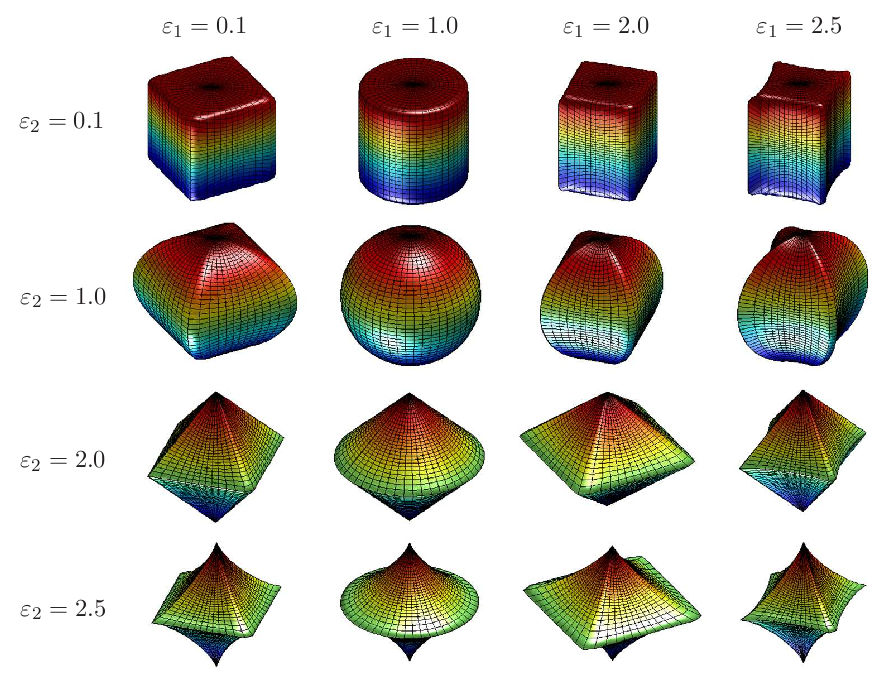
\includegraphics[width=14cm]{./fig_cha3/superquadrics.jpg}
  \caption{Illustration of 3D superquadric shapes with varying rounding parameters\protect\footnotemark.}
  \label{fig:sq}
\end{figure}


\paragraph{Learning grasp distributions for shape primitives}
%\label{cha3:sec4:combine:primitivegraspdistribution:learning}
~\\

With the method described in Section~\ref{cha3:sec2}, we build GMMs for the feasible grasp distributions for a set of shape primitives, i.e. superquadrics. Again, we model the distribution with a GMM as a sum of $K$ Gaussian components:

\begin{equation}
{
P (\boldsymbol{h},\boldsymbol{o},\boldsymbol\theta \text{\textbar} \varOmega)
= \sum_{k=1}^K {p_{k}p(\boldsymbol{h},\boldsymbol{o},\boldsymbol{\theta} \text{\textbar} {\boldsymbol{\mu}_k}, {\boldsymbol{\Sigma}_k})}
}
\end{equation}
where $k$ is the number of Gaussian components, $p_k$ the prior of the Gaussian component and the $\boldsymbol{\mu}_k$, $\boldsymbol{\Sigma}_k$ the corresponding mean and covariance.

Figure~\ref{fig:primtivedistr} visualizes the grasp distributions encoded by GMMs for three shape primitives: a box, a sphere and a cylinder. The robot hand we use here is the Barrett hand.

\begin{figure}
  \centering
    \subfloat[\scriptsize{Box}] {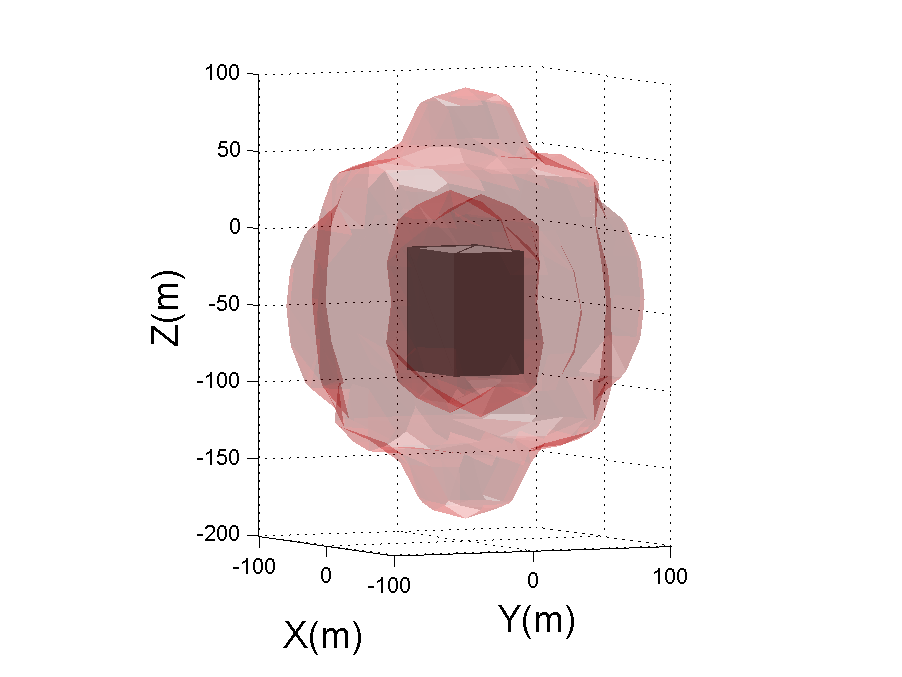
\includegraphics[width=4.5cm]{./fig_cha3/box1.eps}}
    \subfloat[\scriptsize{Sphere}]  {\includegraphics[width=4.5cm]{./fig_cha3/ball2.jpg}}
    \subfloat[\scriptsize{Cylinder}]  {\includegraphics[width=4.5cm]{./fig_cha3/cyl.jpg}}
  \caption{A 3D visualization of the feasible grasp distribution for three shape primitives and the Barrett hand. The red contours are the isosurfaces of the grasp distribution. The ``redder'' the area is, the denser the distribution is.}
  \label{fig:primtivedistr}
\end{figure}


\subsubsection{Combining grasp distribution} ~\\
\label{cha3:sec4:combine:combining}
For an object composed of a few shape primitives, its grasp distribution is the combination of the the grasp distributions of its primitive components. However, this ``combination'' is not a summation of the GMMs: we need to exclude the grasps causing collision.

Before combining the grasp distributions, which are encoded by GMMs, of different shape primitive components of an object, we need to reshape each GMM by the object geometry. This is because when primitives combine to a more complex shape object, the grasp space of one part might be blocked by other part of the object.

For example, an object combined by a cylinder and a sphere is shown in Fig.~\ref{fig:object}(a) and it's primitives with their grasp distributions are shown in (b) and (c). As can be seen in (b) and (c), the top part of the grasp distribution of the cylinder will be inside the sphere and the bottom part of the grasp distribution of the sphere will be inside the cylinder. Grasps generated from these parts will cause collisions between the hand and the object and hence they have to be excluded from the model. 
% Finger collision
%Further, even when the robot hand is placed in a feasible location for all components, when the fingers clutch to grasp one component of the object, the moving trajectory of the finger might be blocked by other components. These kind of grasps should also be excluded from the grasp density of the whole object.
%Therefore, we take into account two kinds of collisions: collisions between the palm and the object and collisions between the finger trajectories and the object. 
To avoid collisions, we use the ``object sigmoid'' function to remove the collision parts.

\paragraph{Object sigmoid} ~\\
\label{cha3:sec4:combine:sigmoid}
We define a shape descriptor ``object sigmoid'' for objects modelled by a superquadric. The object sigmoid is a 3 dimensional sigmoid function defined as:
\begin{equation}
s\left(x, y ,z\right) = \frac{1}{1+e^{-100\left(r\left(x, y ,z\right)-1\right)}}
\label{equ:objectsigmoid}
\end{equation}
where r$\left(x, y ,z\right)$ is a function of the location defined in the form of a superquadrics. When we model an object shape with a superquadric, the object sigmoid has different values inside, on and outside the object:
\begin{equation}
    s
    \begin{cases}
        \rightarrow0, & \text{inside the object}\  \\
        =0.5 & \text{on the surface of the object}\ \\
        \rightarrow1 & \text{outside the object}
    \end{cases}
\end{equation}
In equation~\ref{equ:objectsigmoid} we choose a large coefficient, i.e. 100, for $r$ to make a sharp transition between 0 and 1 and hence a sharp cut on the object surface. Hence the object sigmoid gives a description of the shape of the object in the space: zero inside the object and one outside the object.

Each primitive component has its own object sigmoid. Before combining the individual distributions to form the whole distribution, each individual distribution is multiplied by all other components' object sigmoids. In this way, the likelihood inside the other parts of the object is reduced to zero, while the likelihood outside the object remains. The grasp distribution is hence ``trimmed'' by the other components of the object. The grasp distribution of the whole object is the summation of all the trimmed grasp distributions:

\begin{equation}
\boldsymbol{\Omega}\left(x,y,z\right) = \sum_{i=1,2..}^{N}\left(\Omega_i\prod_{j=1,2..\left(j\neq{i}\right)}^{N}s_j\right)
\end{equation}
where $\Omega_i$, $s_j$, $N$ is the grasp distribution of the $i-th$ primitive component, the object sigmoid of the $j-th$ primitive component and the total number of primitive components. The total number of Gaussians in the GMM of the whole object is the sum of the number of each primitives.

Figure.~\ref{fig:object}(d) shows the resulting grasp distribution of the whole object, which is the combination of the trimmed grasp GMM of the cylinder (Figure.~\ref{fig:object}(d)) and the sphere (Figure.~\ref{fig:object}(f)). Strictly speaking, the combined grasp distribution is not a density function, as the integral of the probability of the whole space is not normalized to one. Despite this, it does not effect the computation of a new grasp as we consider each Gaussian component individually.

\begin{figure}
\centering
    \hspace{-1cm}
    \begin{minipage}[c]{1\textwidth}
    \subfloat[\scriptsize{Novel object}]  {\includegraphics[width=5cm]{./fig_cha3/object.jpg}}
    \subfloat[\scriptsize{Cylinder grasp distribution}] {\includegraphics[width=5cm]{./fig_cha3/cyl.jpg}}
    \subfloat[\scriptsize{Sphere grasp distribution}] {\includegraphics[width=5cm]{./fig_cha3/ball2.jpg}}



    \subfloat[\scriptsize{Combined object grasp distribution}] {\includegraphics[width=5cm]{./fig_cha3/cylball.jpg}}
    \subfloat[\scriptsize{Trimmed grasp distribution}] {\includegraphics[width=5cm]{./fig_cha3/cyl_sig.jpg}}
    \subfloat[\scriptsize{Trimmed grasp distribution}] {\includegraphics[width=5cm]{./fig_cha3/ball_sig2.jpg}}
    \end{minipage}

\caption{\scriptsize{(a) A combination of a cylinder and a sphere. (b) A 3D illustration of the grasp GMM of the cylinder. The red patch is the isosurface of the grasp GMM. (c) The grasp GMM of the sphere. (d) The combined grasp GMM of the whole object (d={e,f})). (e) The trimmed grasp GMM of the cylinder. The top part of the GMM is removed. (f) The trimmed grasp GMM of the sphere. Part of the bottom of the GMM is removed.}}
\label{fig:object}
\end{figure}


The equation above removes the grasps inside the object and hence avoids the collision between the robot palm and the object. 

% Finger collision
%However, grasps causing collision between finger trajectory and the object still remain.
%\paragraph{TODO: Trim grasp distribution by finger trajectory} ~\\


\subsection{Plan Grasp by combined grasp distribution}
\label{cha3:sec4:plan}

With the combined grasp distribution for the whole object, we can fast plan a grasp with the method described in Section~\ref{cha3:sec2}. Starting from an initial hand position and orientation $q = \{h, o\}$, the first step to compute a new grasp is to project $q$ to the feasible region of the GMM, where the probability of finding a stable grasp is high. This is done by finding the minimum Mahalanobis distance between $q$ and its projection point $q_k^\star$ in each Gaussian component of the GMM.

The projection point $q_k^{\star}$ of the $k$-th Gaussian component is computed as:
\begin{equation} \label{alpha}
q_k^{\star} = q + \alpha_k\left(q-\mu_k\right)
\end{equation}
where $\mu_k$ is the mean of the $k$-th Gaussian and $\alpha_k$ is a scalar determined by the boundary of the feasible region.

For $q_k^{\star}$ we have
\begin{equation} \label{qstar}
-\frac{1}{2}\left(q_k^{\star}-\mu_k\right)^T\Sigma_k^{-1}\left(q_k^\star-\mu_k\right)=-\frac{1}{2}\cdot{1}^{2}
\end{equation}
with equation~\ref{alpha} and~\ref{qstar}, $\alpha_k$ can be computed and hence $q_k^{\star}$.

The feasibility of each projection point is checked by the object sigmoids:

\begin{equation}
l_k = \prod_{j=1,2,...\left(j\neq{k}\right)}^N{s_j}
\end{equation}
If $l_k$ is smaller than 1, indicating that this point is inside or on the surface of the object, the likelihood at point $q^{\star}_k$ is zero.

We find the nearest projection point from the $q_k^\star$ with non-zero density. The nearest $q_k^\star$ is chosen to be the final grasp hand position and orientation $q^\star$. The grasp distribution $\Omega^{\star}$ which $q^{\star}$ locates in is used to compute the corresponding joint configuration though GMR. This allows us to compute the expected value of the finger joints from the conditional $p\left(\theta\mid{q^{\star}},\Omega^{\star}\right)$ (Section~\ref{cha3:sec2}). 
\section{Experiments of planning grasps for non-familiar objects}
\label{cha3:sec5}


\begin{table*}
\renewcommand{\arraystretch}{1.5}
\centering
\caption{Success rate and computation time of different methods and objects}
%\hspace{-2cm}
    \begin{tabular}
    { |>{\centering\arraybackslash}p{4cm}  | >{\centering\arraybackslash}p{2cm} | >{\centering\arraybackslash}p{3cm} |  >{\centering\arraybackslash}p{2cm} |  >{\centering\arraybackslash}p{2cm} |}
    \hline
    Approach and object & Force-Closure Grasp Found &  Mean of Computation Time($msec$) & Variance ($msec$)   \\ \hline
    Pre-trained grasp GMM for the novel object       & 98.1\%  & 13.8    & 0.015 \\ \hline
    Combined grasp GMM for novel object             & 92.1\%  & 21.9    & 0.011 \\ \hline
    Combined grasp GMM for spray flask              & 91.0\%  & 16.0    & 0.004 \\ \hline
    Combined grasp GMM for bedside table            & 82.2\%  & 21.1    & 0.006 \\ \hline
    \end{tabular}

\label{tab:result}
\end{table*}

\begin{table*}[ht!]
\renewcommand{\arraystretch}{1.5}
\centering
\caption{Shape primitives used in experiments}
%\hspace{-2cm}
    \begin{tabular}
    %{ | c | c | c |>{\centering\arraybackslash}p{3cm} |>{\centering\arraybackslash}p{3cm}|}
    {|>{\centering\arraybackslash}p{2cm}|>{\centering\arraybackslash}p{2.5cm}|>{\centering\arraybackslash}p{3cm}|>{\centering\arraybackslash}p{1.5cm} |>{\centering\arraybackslash}p{1.5cm}|}
    \hline
    Shape primitives& Object & Size($cm$) & Amount of training data & Number of Gaussians in GMM   \\ \hline
    Sphere 1        & Novel object (Fig.~\ref{fig:object})  & radius 7              & 12096    & 60 \\ \hline
    Cylinder 1      & Novel object (Fig.~\ref{fig:object})  & height 15 and radius 4& 15608    & 60 \\ \hline
    Box 1 & Spray flask (Fig.~\ref{fig:spr})        & $6\times9.5\times8$       & 9256    & 40 \\ \hline
    Box 2 & Spray flask (Fig.~\ref{fig:spr})        & $4\times11\times4.5$      & 7544    & 40 \\ \hline
    Box 3 & Spray flask (Fig.~\ref{fig:spr})        & $2.5\times4\times7$       & 3400    & 30 \\ \hline
    Box 4 & Bedside table (Fig.~\ref{fig:bedside})  & $52.5\times3\times52.5$   & 8668    & 20 \\ \hline
    Box 5 & Bedside table (Fig.~\ref{fig:bedside})  & $2.8\times57.6\times2.7$  & 4392    & 20 \\ \hline
    \end{tabular}

\label{tab:primitive}
\end{table*}

We test our approach initially on a novel object that is a combination of a sphere and a cylinder (Figure.~\ref{fig:object}(a) and Table~\ref{tab:primitive}). We choose to use the Barrett hand for the implementation as it is available in our lab. As explained above, the grasp of the Barrett hand is formulated as the combination of the hand position ($h$), orientation($o$) and finger joint angles($\theta$).  The grasp GMMs of the sphere and cylinder are pre-trained with randomly generated stable grasps from the simulator GraspIt!.

We compare this new approach with the previous approach that directly trained a grasp GMM for the whole object, by generating grasps for the object from 1000 starting points. Figure.~\ref{fig_result} shows a few resulting grasps. As shown in the Table~\ref{tab:result}, the success rate and the computation time of the new approach is of the same scale as the previous approach. The computation time is computed by Matlab on the same machine we use for the experiments described in Section~\ref{cha3:sec3} ( with a 2.8GHz processor and a 4GB RAM).


Further, we train 5 different boxes as our primitives (Table~\ref{tab:primitive}) and use them to approximate two daily life objects: a spray flask and a bedside table. The spray flask is approximated as the combination of box 1, 2 and 3 (Figure.~\ref{fig:spr}) and the bedside table is approximated as the combination of box 4 and 5 (three copies of box 4 as the surfaces and 4 copies of box 5 as the legs). The result is shown in Table~\ref{tab:result}. A few initial hand postures and their resulting grasps are shown in Figure~\ref{fig:spr_result} and~\ref{fig:result:bedside}.

%\vspace{-0.2in}
\begin{figure}[!ht]
%\vspace{-0.3cm}
\centering
    \subfloat[  {Initial pose 1}]  {\includegraphics[width=4.5cm]{./fig_cha3/8_i.jpg}}
    %\hspace{-0.01in}
    \subfloat[  {Initial pose 2}] {\includegraphics[width=4.5cm]{./fig_cha3/1_i.jpg}}
    %\hspace{0.01in}
    \subfloat[  {Initial pose 3}] {\includegraphics[width=4.5cm]{./fig_cha3/5_i.jpg}}
    %\vspace{0.05in}

    \subfloat[  {Final grasp 1}] {\includegraphics[width=4.5cm]{./fig_cha3/8_f.jpg}}
    \hspace{0.005in}
    \subfloat[  {Final grasp 2}] {\includegraphics[width=4.5cm]{./fig_cha3/1_f.jpg}}
    \hspace{0.005in}
    \subfloat[  {Final grasp 3}] {\includegraphics[width=4.5cm]{./fig_cha3/5_f.jpg}}

    \subfloat[  {3D projections}] {\includegraphics[width=7cm]{./fig_cha3/object_cylball_i_f_arrow.jpg}}
    \hspace{0.005in}
    \subfloat[  {2D contour projections}] {\includegraphics[width=6cm]{./fig_cha3/contour_Z_cylball_i_f_arrow2.jpg}}

\caption{  {Examples of Barrett hand grasping of a novel object. (a-d) Initial hand postures and final grasps. (g) A 3D illustration of the projection between the initial hand postures and the final grasps. (h) a 2D illustration of the interaction of GMM at $z$ = 0.}}

%\vspace{-0.2cm}
\label{fig_result}
\end{figure}

\begin{figure}
\centering
    \subfloat[  {}]  {\includegraphics[width=5cm]{./fig_cha3/spr.jpg}}
    \hspace{1cm}
    \subfloat[  {}] {\includegraphics[width=5cm]{./fig_cha3/box123.jpg}}
%    \hspace{0.01in}
\caption{  {(a) A spray flask. (b) A spray flask approximated by 3 boxes.}}
\label{fig:spr}
\end{figure}



\begin{figure}[!ht]
\centering
    \subfloat[  {Initial pose 1}]  {\includegraphics[height= 3cm]{./fig_cha3/spr_3_i.jpg}}
    \hspace{0.3cm}
    \subfloat[  {Initial pose 2}] {\includegraphics[height= 4cm]{./fig_cha3/spr_4_i.jpg}}
    \hspace{0.3cm}
    \subfloat[  {Initial pose 3}] {\includegraphics[height= 4cm]{./fig_cha3/spr_6_i.jpg}}

    %\vspace{0.05in}
    \subfloat[  {Final grasp 1}] {\includegraphics[width=4cm]{./fig_cha3/spr_3_f.jpg}}
    \hspace{1.5cm}
    \subfloat[  {Final grasp 2}] {\includegraphics[height=4cm]{./fig_cha3/spr_4_f.jpg}}
    \hspace{0.3cm}
    \subfloat[  {Final grasp 3}] {\includegraphics[width=4cm]{./fig_cha3/spr_6_f.jpg}}

\caption{  {Examples of Barrett hand grasping of a spray flask. }}
%\vspace{-0.8cm}
\label{fig:spr_result}
\end{figure}


\begin{figure}
\centering
    \subfloat[  {}]  {\includegraphics[width=5cm]{./fig_cha3/bedside.jpg}}
    \hspace{0.07in}
    \subfloat[  {}] {\includegraphics[width=5cm]{./fig_cha3/bedside_box.jpg}}
%    \hspace{0.01in}
\caption{  {(a) A bedside table. (b) A bedside table approximated by 7 boxes.}}
\label{fig:bedside}
\end{figure}

\begin{figure}
\centering
    \subfloat[  {Initial pose 1}]  {\includegraphics[width=4cm]{./fig_cha3/bed_6_i.jpg}}
    \hspace{0.2cm}
    \subfloat[  {Initial pose 2}] {\includegraphics[width=4cm]{./fig_cha3/bed_3_i.jpg}}
    \hspace{0.7cm}
    \subfloat[  {Initial pose 3}] {\includegraphics[width=4cm]{./fig_cha3/bed_5_i.jpg}}
    %\vspace{0.05in}

    \subfloat[  {Final grasp 1}] {\includegraphics[width=4cm]{./fig_cha3/bed_6_f.jpg}}
    \hspace{0.005in}
    \subfloat[  {Final grasp 2}] {\includegraphics[width=4cm]{./fig_cha3/bed_3_f.jpg}}
    \hspace{0.005in}
    \subfloat[  {Final grasp 3}] {\includegraphics[width=4cm]{./fig_cha3/bed_5_f.jpg}}


\caption{  {Examples of Barrett hand grasping of a complex shape bedside table (a-d) Initial hand postures and final grasps. }}
\label{fig:result:bedside}
\end{figure}


%$\bullet$ TODO: grasp density can be used to find grasps by task (Detry)
%$\bullet$ TODO: can not find grasps over different parts
%$\bullet$ TODO: interpolate primitives?
%$\bullet$ TODO: human spend more time on new object
%$\bullet$ TODO: take volume of robot hand into account
%In implementation we found the success rate depends on how well we can approximate the novel object with known shape primitives, and hence the choice of the shape primitives is important.Future work will focus on studying how to interpolate the grasp GMM for different shape primitives, to allow the novel objects to be approximated more precisely.


\section{Discussion}
\label{cha3:sec6:discussion}

We presented a method for computing grasps in real time. This is demonstrated on two very different robot platforms: the iCub hand and the Barrett hand. The result shows that the method can capture the versatility of grasps that are typical of grasps performed by an industrial gripper, and those that can be performed by a humanoid hand.
With the computation time in the millisecond scale,
this method would enable the robot to react quickly in robot-human interaction, such as picking up heavy objects from a person's hand, as well as adopting to fast perturbations in a dynamic environment.

We achieve this goal by using a closed-form solution. A GMM model is learned from the grasping demonstration generated offline for a given object. During the online execution no iterative method is used, we only need to solve a few equations with basic arithmetic operations. Hence the computation time is significantly shorter than the conventional optimization methods. Though we need to pre-train the robot to grasp different objects, in many scenarios such as surgery assistance, robots and humans must work with a predefined set of objects. This allows us to build the grasping model for each object beforehand.


To find the closest Gaussian component we used the Mahalanobis distance rather than the Euclidean distance. The advantage of this is that it takes into account the correlations among each dimension of the hand configuration. In a space of different types of measurements, i.e. length and angle, Mahalanobis space is a better representation than the Euclidean space. Indeed, humans do not always use the Euclidean distance to select their grasps. We may move our hand further than needed to grasp an object, in order to avoid flipping our hand to another orientation.

Our approach provides a good estimation of a stable and feasible grasp for the given object and robot hand. To model the actual contact points between the robot hand and the object is difficult in real time because of the high dimension of the solution space and the non-linearity of the kinematic constraints. In our method, instead of computing the actual contact point position, we compute the most likely solution using a GMM. Though a certain amount of accuracy is traded off to achieve the real time goal, the overall performance is satisfying. In our experiments, over 90 percent of the testing points find good grasps within a few milliseconds. This method is most efficient for objects with a smooth surface. For complex objects this method can achieve a high success rate of over 85\%. When grasping the parts requiring high precision, additional feedback from visual or tactile sensors is needed for further refinement of the grasp.

When extending this approach to grasp non-familiar objects, we exploit an modular approach: grasp by shape primitives. The grasp distribution is learnt for each shape primitive and is combined to form the distribution for the whole object. Experiments show that this method enable the robot to grasp complex objects with high successful rate (over 80\%) while maintaining the computation time with in millisecond scale. 

%The way we project the initial query point to the closest Gaussian component is more conservative.
In contrast to the common approach of learning from human demonstrations,
these grasps are generated solely according to the mechanics of the robot hand.
Some resulting grasps are markedly different from  human grasps, especially for the Barrett hand which is very different from the human hand.
Our method may therefore out perform human demonstrations in some
contexts by better exploiting differences between human and robot ``physiology''. 




